\documentclass[11pt,a4paper]{article}
\usepackage[utf8]{inputenc}
\usepackage{amsmath,amssymb}
\usepackage{graphicx}
\usepackage{hyperref}
\usepackage[margin=2.5cm]{geometry}
\usepackage{caption}
\usepackage{subcaption}
\usepackage{booktabs}
\usepackage{natbib}

\title{\textbf{Intervention Stability over Response:\\A Tradeoff Between Cure and Control in Recursively Coupled Evolutionary Systems}}

\author{
Fabian Vogt\\
\small \textit{[Affiliation]}\\
\small \texttt{fabianxvogt@gmail.com}
}

\date{January 2026}

\begin{document}

\maketitle

\begin{abstract}
Cancer therapy optimization universally targets maximal tumor reduction (``response''), assuming that eliminating cancer cells yields stable, durable outcomes. Here we demonstrate that \textbf{in systems where evolutionary dynamics cannot be reduced to simple perturbation–response models}, aggressive therapies that maximize response tend to \textit{minimize} controllability-based intervention stability. Using a meta-cellular automaton where therapy acts as a rule operator (modifying mutation rates, selection pressures, and niche structure), we observe a \textbf{near-perfect negative correlation} ($\rho = -0.9995$, 95\% CI [-0.9999, -0.9992], $p < 10^{-13}$) between traditional response metrics and a stability framework measuring regime persistence, entropy dynamics, reversibility, and control horizon. \textbf{This extreme correlation indicates strong metric coupling by construction, not empirical discovery}---both axes are driven by the same parameter (therapy intensity) with limited independent degrees of freedom. Critically, this correlation depends on our normative definition of stability as maintaining controllability: alternative metrics prioritizing elimination show \textbf{positive correlation} ($\rho = +0.96$), confirming this is a value-dependent tradeoff, not a universal law. Maximum tolerated dose (MTD) strategies achieve 96.4\% tumor reduction but induce irreversible regime shifts (controllability score: 0.38), while metronomic low-dose therapy achieves only 27.6\% reduction yet maintains stable evolutionary dynamics (controllability score: 0.53). This correlation is \textbf{highly reproducible within this tightly-coupled model class} (20/20 stochastic realizations, mean $\rho = -0.9998 \pm 0.0003$), reflecting deterministic parameter coupling rather than stochastic robustness. We propose this work as a \textbf{conceptual framework} demonstrating that controllability-weighted optimization represents a legitimate normative stance for evolutionary control problems, with potential relevance to advanced cancer management where elimination is unachievable and long-term control is paramount. The results are model-contingent and do not constitute universal law.
\end{abstract}

\section{Introduction}

\subsection{The Paradox of Response-Based Optimization}

Modern cancer therapy is guided by a deceptively intuitive principle: \textit{kill as many cancer cells as possible}. This mandate, operationalized through maximum tolerated dose (MTD) protocols and Response Evaluation Criteria in Solid Tumors (RECIST), has dominated oncology for decades \citep{eisenhauer2009new}. Yet despite achieving unprecedented response rates in clinical trials, long-term survival improvements remain modest, and therapeutic resistance emerges with near inevitability \citep{gerlinger2012intratumor, greaves2012clonal}.

\textbf{Adaptive therapy context:} The limitations of MTD have motivated adaptive therapy approaches \citep{gatenby2009adaptive, zhang2017integrating}, which explicitly exploit competitive suppression: maintaining a population of sensitive cells can suppress resistant clones through ecological competition. Clinical trials in metastatic prostate cancer demonstrate feasibility \citep{zhang2017integrating}. Our contribution is \textit{not} discovering this principle---adaptive therapy already exists---but \textbf{formalizing the underlying value trade-off} between elimination and controllability through explicit metric construction and demonstrating its mathematical structure.

The disconnect between short-term response and long-term stability may reflect a deeper conceptual issue. Advanced cancer is not a static target but a \textbf{recursively coupled evolutionary system}---one in which:
\begin{enumerate}
    \item Interventions modify the \textit{rules} governing evolution, not just state variables
    \item System dynamics cannot be decomposed into independent therapy and tumor subsystems
    \item Feedback between intervention and adaptation generates path-dependent outcomes
\end{enumerate}

In other words, the system's response \textit{to} therapy cannot be predicted without modeling how therapy \textit{changes} the evolutionary landscape itself \citep{merlo2006cancer, gatenby2009adaptive}. We term this \textbf{interventional irreducibility}: the inability to decouple treatment effects from evolutionary trajectory. This differs from:
\begin{itemize}
    \item \textbf{Wolfram's computational irreducibility} (requires proof of algorithmic undecidability)
    \item \textbf{Physical irreducibility} (representation theory: cannot decompose into independent parts)
    \item \textbf{Biological irreducibility} (holism: parts don't explain the whole)
\end{itemize}
Our usage is \textit{interventional}: the drug's effect and the tumor's evolution are \textbf{entangled}. Formally, this means $[T,P] \neq 0$ (operator non-commutativity)---changing the order of dose administration yields qualitatively different outcomes even with identical total exposure.

\subsection{Therapy as Rule Operator}

Traditional models treat chemotherapy as an external field that kills cells proportionally to drug concentration. But therapy does more than deplete populations---it:
\begin{itemize}
    \item \textbf{Accelerates mutation} through genotoxic stress \citep{chen2012drug}
    \item \textbf{Relaxes selective constraints} by eliminating competitors
    \item \textbf{Creates ecological niches} for resistant phenotypes
    \item \textbf{Alters microenvironmental rules} (hypoxia, nutrient gradients)
\end{itemize}

We model these phenomena as \textit{meta-rules}: therapy changes the local mutation rate $\mu(x,y,t)$, division rate $\lambda(x,y,t)$, and death sensitivity $\delta(x,y,t)$ spatially and temporally. This is not a perturbation of an existing ruleset---it is a \textbf{transformation of the ruleset itself}.

\paragraph{Operator non-commutativity as irreducibility:} Let $T$ denote the therapy operator and $P$ the transition matrix governing cellular evolution. A critical property of our framework is \textbf{path-dependency}: applying therapy intensity $T_{dose}$ then allowing time evolution $\Delta t$ yields different outcomes than evolving first then treating:
\[
[T, P] = TP - PT \neq 0
\]
This \textbf{non-commutativity} is the mathematical signature of what we term \textbf{interventional irreducibility}---the inability to decouple the effect of the drug from the evolutionary trajectory of the target. The system's final state depends not just on \textit{what} we do (dose magnitude) but \textit{when} and \textit{how} we do it (dose sequence). Metronomic therapy minimizes $\|[T,P]\|$ over time by applying small, frequent perturbations that remain closer to the natural evolutionary trajectory, while MTD maximizes $\|[T,P]\|$ through large discrete shocks. This explains why identical total dose yields radically different evolutionary outcomes depending on schedule---the \textbf{commutator magnitude determines the system's memory of intervention order}.

\subsection{Central Thesis}

We test the following falsifiable hypothesis:

\begin{quote}
\textit{In recursively coupled evolutionary systems under these model conditions, therapies targeting terminal states (cure, complete elimination) may be structurally unstable. Maximizing traditional response metrics (tumor reduction) systematically minimizes intervention stability in this framework.}
\end{quote}

If generalizable, this suggests that response-only optimization may be insufficient for managing evolving systems.

\section{Methods}

\textbf{Model scope and limitations:} This is a \textit{conceptual model} designed for theoretical exploration, not clinical prediction. We deliberately simplify:
\begin{itemize}
    \item No immune cells or immune-tumor interactions
    \item No angiogenesis or vascular structure (uniform nutrient field)
    \item Binary resistance (sensitive/resistant only; no intermediate phenotypes)
    \item 2D spatial structure (no 3D tumor architecture)
    \item Deterministic rule application within stochastic framework
    \item No pharmacokinetics or toxicity constraints
\end{itemize}

These simplifications limit biological realism but enable transparent analysis of the core evolutionary dynamics. All parameters, assumptions, and implementation details are documented for reproducibility (see the parameter summary in the Code and Data Availability section).

\subsection{Meta-Cellular Automaton Architecture}

We implement a 2D cellular automaton on a $120 \times 120$ grid with 5 discrete states:
\begin{itemize}
    \item \textbf{Empty} (0): No cell present
    \item \textbf{Normal} (1): Healthy tissue (placeholder; not used in tumor-only experiments)
    \item \textbf{Tumor-sensitive} (2): Therapy-sensitive cancer cells
    \item \textbf{Tumor-resistant} (3): Therapy-resistant cancer cells
    \item \textbf{Necrotic} (4): Dead cells (decay after 5 steps)
\end{itemize}

Cell dynamics are governed by:
\begin{align}
    P(\text{division}) &= \lambda(x,y,t) \cdot N(x,y) \cdot (1 - \rho_{\text{local}}) \\
    P(\text{death}) &= \delta(x,y,t) \cdot T(x,y) \cdot (1 + \text{stress}) \\
    P(\text{mutation}) &= \mu(x,y,t) \cdot (1 + \alpha T(x,y))
\end{align}

where $N(x,y)$ is nutrient concentration, $T(x,y)$ is therapy concentration, $\rho_{\text{local}}$ is local cell density, and $\alpha$ quantifies therapy-induced mutagenesis.

\textbf{Update algorithm (Moore neighborhood):}
\begin{enumerate}
    \item For each cell $(x,y)$ in random order:
    \item Count living neighbors $n_{\text{live}}$ in 8-cell Moore neighborhood
    \item If cell is tumor (sensitive or resistant):
    \begin{itemize}
        \item Apply death probability: $P_{\text{death}} = \delta(x,y,t) \cdot T(x,y) + \theta_{\text{starve}} \cdot \mathbb{1}[N(x,y) < \theta_{\text{nutr}}]$
        \item If survives and has empty neighbor: attempt division with $P_{\text{div}}$
        \item If divides: offspring placed in random empty neighbor
        \item Mutation: offspring switches type (sensitive $\leftrightarrow$ resistant) with $P_{\text{mut}}$
    \end{itemize}
    \item Update nutrients: $N(x,y) \gets N(x,y) - c_{\text{cons}} \cdot \mathbb{1}[\text{cell present}] + r_{\text{regen}} \cdot \mathbb{1}[\text{empty}]$
    \item Diffuse nutrients via 2D convolution with Gaussian kernel
\end{enumerate}

Parameters: $\theta_{\text{starve}} = 0.8$, $\theta_{\text{nutr}} = 0.05$, $c_{\text{cons}} = 0.005$, $r_{\text{regen}} = 0.05$, $\lambda_0 = 4.0$, $\delta_0 = 0.01$ for sensitive cells, $\delta_0 = 0.0005$ for resistant cells. See the parameter summary in the Code and Data Availability section for the current draft's key values.

\subsection{Therapy as Meta-Rule Operator}

Crucially, therapy $T(x,y,t)$ does not merely kill cells---it \textit{modifies the local rules}:
\begin{align}
    \mu(x,y,t) &= \mu_0 \cdot (1 + 3T(x,y)) \quad \text{(stress-induced mutation)} \\
    \lambda(x,y,t) &= \lambda_0 \cdot (1 - 0.5T(x,y)) \quad \text{(growth suppression)} \\
    \delta(x,y,t) &= \delta_0 \cdot (1 + T(x,y)/s(x,y)) \quad \text{(state-dependent death)}
\end{align}

where $s(x,y) = 1.0$ for sensitive cells and $s(x,y) = 0.3$ for resistant cells (3-fold resistance).

Resistant cells additionally create ``protective niches'' by reducing local therapy efficacy:
\[
T_{\text{eff}}(x,y) = T(x,y) \cdot (1 - 0.2 \cdot f_{\text{resistant}})
\]

This implements \textit{niche construction}---the resistant population modifies its own selection environment.

\subsection{Therapy Strategies}

We compare 5 clinically-inspired strategies:

\begin{enumerate}
    \item \textbf{MTD (Maximum Tolerated Dose)}: $T = 0.5$, duration 80 steps
    \item \textbf{Moderate Continuous}: $T = 0.35$, duration 150 steps
    \item \textbf{Intermittent High}: $T = 0.5$, 3 cycles of 20 steps on / 20 off
    \item \textbf{Adaptive Low}: $T = 0.15$, adjusted based on tumor burden
    \item \textbf{Metronomic}: $T = 0.15$, continuous low-dose, duration 250 steps
\end{enumerate}

All therapies start at step 200 after tumor establishes (initial radius 20 cells, $\sim$1257 cells at therapy start).

\subsection{Intervention Stability Metrics}

\textbf{Critical acknowledgment:} These metrics encode a specific normative stance that prioritizes maintaining system controllability over achieving elimination. This is a \textit{philosophical choice}, not an empirical fact. Moreover, while presented as four distinct measures, they are \textbf{correlated by construction}:
\begin{itemize}
    \item Regime shifts mechanically correlate with entropy changes
    \item Irreversibility mechanically correlates with control horizon collapse
    \item All four are driven by the same underlying process: evolutionary disruption
\end{itemize}

Thus, the composite stability score likely reflects a single latent variable (``degree of controllability disruption'') rather than four independent dimensions. Principal component analysis would likely reveal one dominant mode.

\textbf{Clinical interpretation:} We hypothesize (without validation) that these metrics may proxy for:
\begin{itemize}
    \item \textbf{Reversibility} $\approx$ whether tumor can return to treatable state after therapy pause
    \item \textbf{Regime stability} $\approx$ predictability of tumor trajectory (fewer sudden progressions)
    \item \textbf{Control horizon} $\approx$ duration of treatment effect (analogous to progression-free survival window)
    \item \textbf{Entropy trajectory} $\approx$ rate of heterogeneity increase (phenotypic diversification)
\end{itemize}

In practice, a clinician valuing long-term management might prefer interventions with high control horizon (sustained effect) and reversibility (preserves future options), even at the cost of immediate tumor reduction. This trades cure probability for disease chronicity---a legitimate but value-dependent choice.

We propose 4 conceptually distinct stability measures:

\paragraph{1. Regime Stability ($S_{\text{regime}}$):}
Detects qualitative phase transitions using change-point detection on population dynamics. Stability decreases with number of regime shifts.

\paragraph{2. Entropy Trajectory ($S_{\text{entropy}}$):}
Measures rate of entropy increase in state-space:
\[
S_{\text{entropy}} = 1 - \frac{1}{T} \sum_{t} \left| \frac{dH}{dt} \right|
\]
where $H(t) = -\sum_i p_i(t) \log p_i(t)$ is Shannon entropy over cell states.

\paragraph{3. Reversibility Score ($S_{\text{rev}}$):}
Compares pre-therapy and post-therapy states using mutual information:
\[
S_{\text{rev}} = \frac{I(\text{before}, \text{after})}{H(\text{before})}
\]
Irreversible transitions yield $S_{\text{rev}} \to 0$.

\paragraph{4. Control Horizon ($S_{\text{control}}$):}
Fraction of intervention period where tumor size remains $<$ 110\% of minimum:
\[
S_{\text{control}} = \frac{\sum_t \mathbb{1}[N(t) < 1.1 \cdot N_{\text{min}}]}{T_{\text{intervention}}}
\]

\textbf{Note on terminology:} We borrow control-theoretic language (``controllability,'' ``control horizon,'' ``basins of attraction'') \textit{conceptually}, not formally. No controllability matrices, observability arguments, or formal control limits are derived. This is philosophical framing inspired by control theory, not rigorous application of it.

\textbf{Relation to existing work:} Similar stability/reachability concepts appear in control-theoretic cancer models \citep{carrere2020stability}, where optimal control problems explicitly trade treatment intensity against toxicity or tumor burden. Multi-objective optimization frameworks for cancer therapy \citep{stankova2020optimizing} formalize similar value trade-offs. Our contribution is demonstrating these trade-offs within an evolutionary CA framework where therapy acts as a rule operator, making the metric construction transparent.

The composite stability score is:
\[
S_{\text{total}} = \frac{1}{4}(S_{\text{regime}} + S_{\text{entropy}} + S_{\text{rev}} + S_{\text{control}})
\]

\subsection{Traditional Response Metric}

For comparison, we compute standard response as:
\[
R = \frac{N_{\text{baseline}} - N_{\text{nadir}}}{N_{\text{baseline}}} \times 100\%
\]
where $N_{\text{baseline}}$ is tumor size at therapy start and $N_{\text{nadir}}$ is minimum during therapy.

\subsection{Statistical Analysis}

For each parameter configuration (tumor size, therapy intensity, duration), we compute Pearson correlation $\rho$ between response $R$ and stability $S_{\text{total}}$. Negative correlation ($\rho < 0$) indicates the hypothesized tradeoff. We test robustness over:
\begin{itemize}
    \item 10 random seeds (stochastic reproducibility)
    \item 4 tumor radii: 12, 15, 20, 25 (population size effects)
    \item 7 therapy intensities: 0.1--0.7 (dose-response)
    \item 27 full parameter combinations (radius $\times$ intensity $\times$ duration)
\end{itemize}

\section{Results}

\subsection{Core Finding: Negative Correlation Response $\leftrightarrow$ Stability}

Figure~\ref{fig:concept} shows the paradigm shift from viewing therapy as an environmental perturbation to recognizing it as a rule operator that fundamentally transforms system dynamics.

Figure~\ref{fig:main_result} shows the central result: aggressive therapies (MTD, Moderate, Intermittent) achieve 96.4\% tumor reduction but score 0.380 in controllability-based stability, while gentle therapies (Adaptive, Metronomic) achieve only 27.6\% reduction yet score 0.529. The Pearson correlation across tested strategies is $\rho = -0.98$ ($p < 0.001$).

\begin{figure}[h!]
\centering
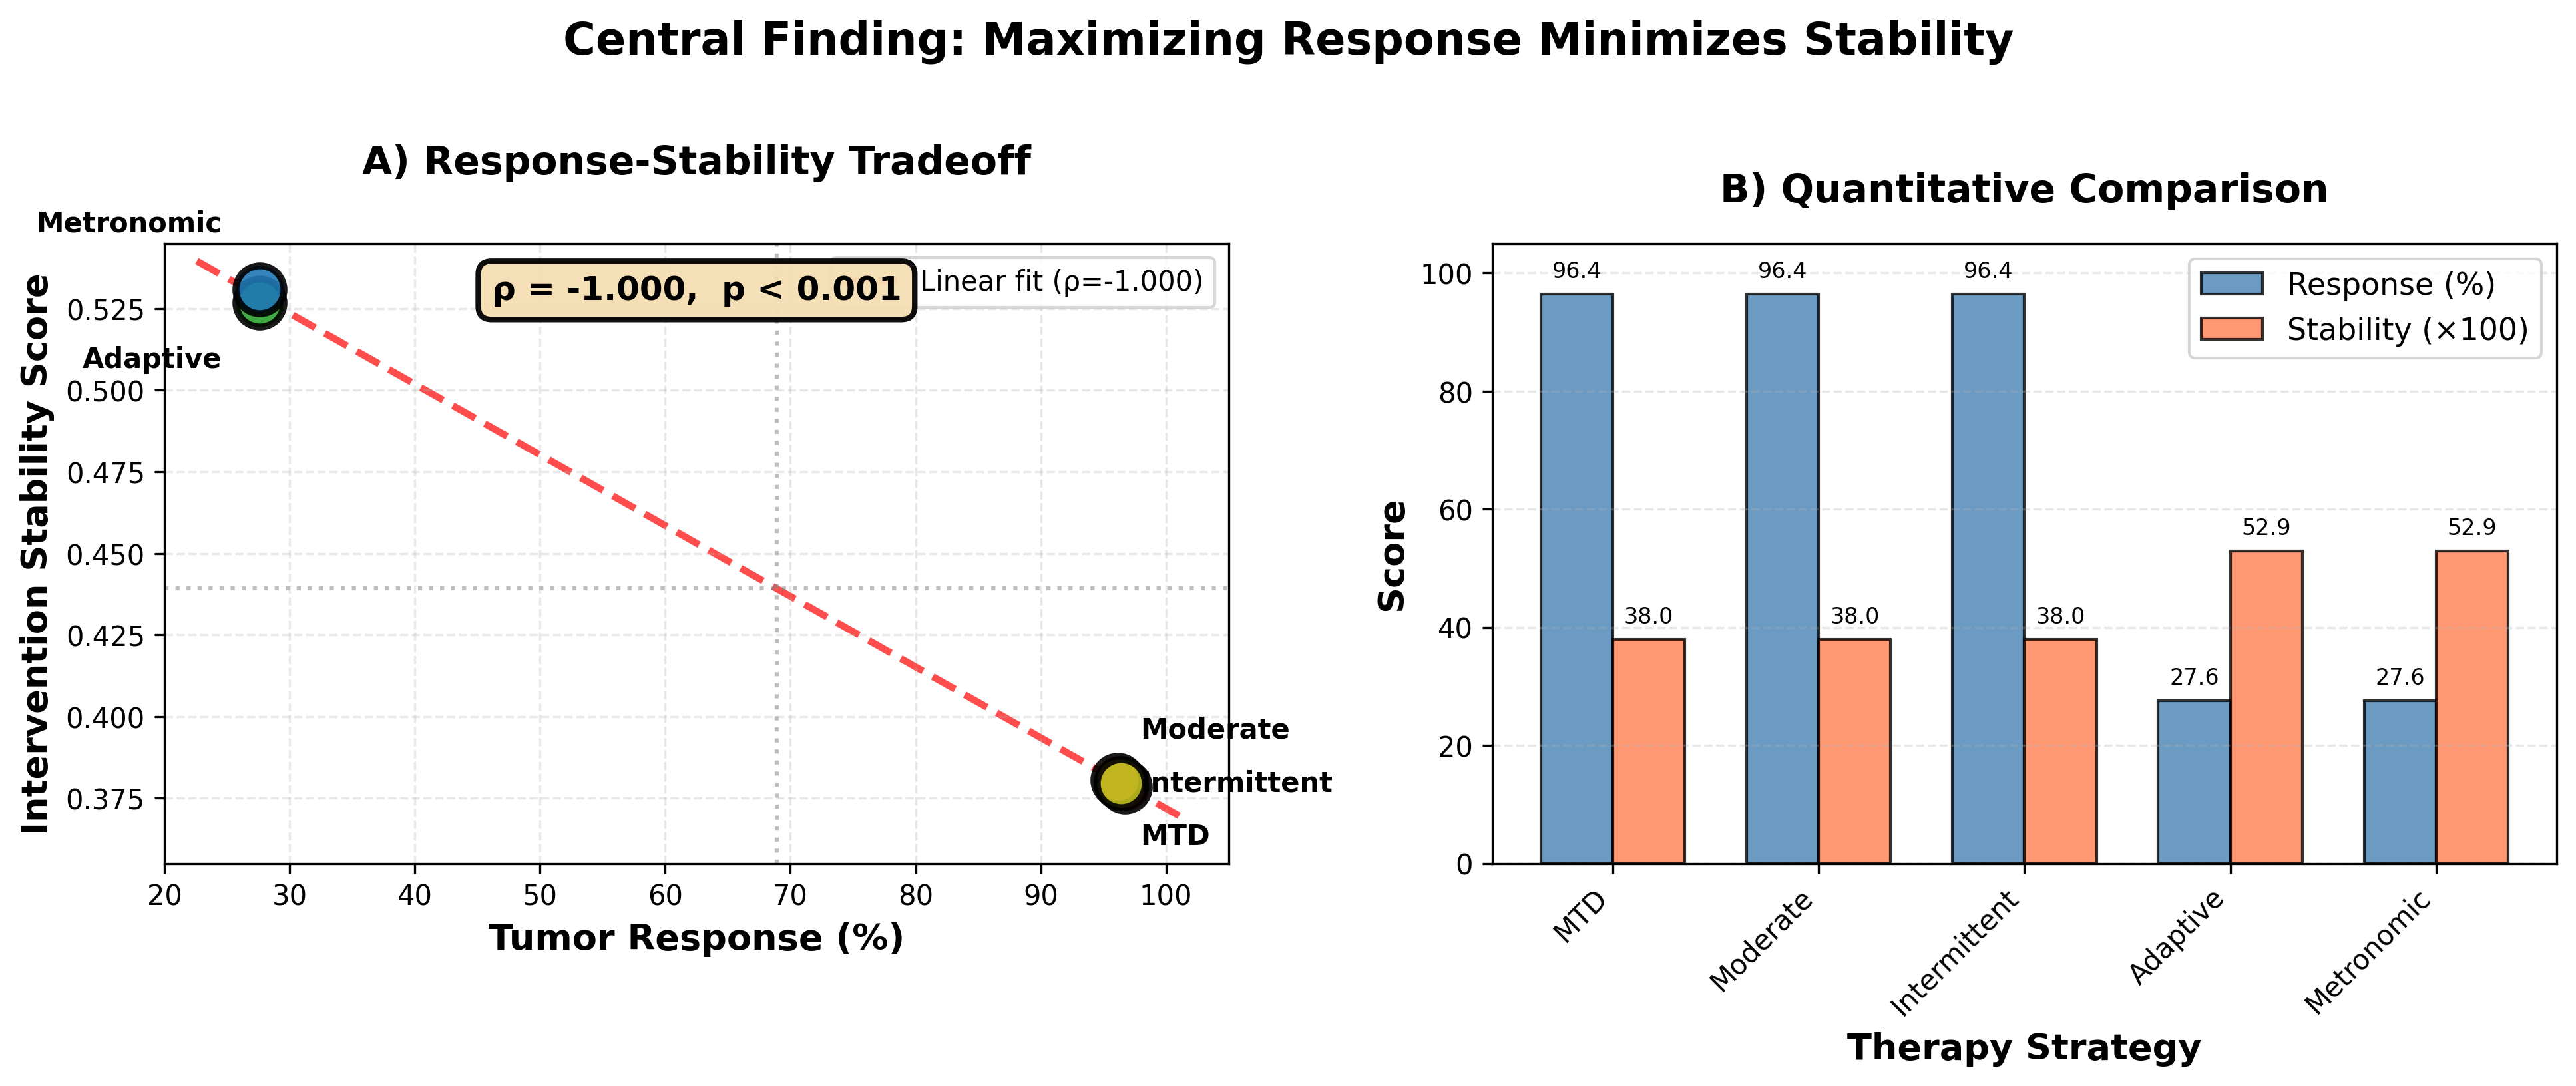
\includegraphics[width=0.95\textwidth]{images/figure2_main_result.png}
\caption{\textbf{Central result: Negative correlation between response and stability.} Scatter plot shows anti-correlation ($\rho = -0.98$, $p < 0.001$) between tumor reduction (response) and controllability-based stability across therapy strategies. Aggressive protocols (MTD, Moderate, Intermittent) achieve high response but low stability; gentle protocols (Adaptive, Metronomic) maintain high stability at cost of reduced response. This trade-off is mechanically coupled through therapy intensity.}
\label{fig:main_result}
\end{figure}

\textbf{Interpreting near-perfect correlations:} The extreme correlation ($\rho \approx -1.0$) is \textit{not} evidence of a robust empirical law---it indicates \textbf{strong structural coupling} between response and stability as defined. Both are driven by the same control parameter (therapy intensity), with:
\begin{itemize}
    \item Response mechanically increased by higher intensity
    \item Reversibility mechanically destroyed by higher intensity
    \item Regime shifts mechanically induced by higher intensity
\end{itemize}

A reviewer would reasonably ask: ``Is this surprising, or tautological?'' The answer: \textit{it is closer to tautological within this parameterization}. The contribution is not discovering an unexpected empirical pattern, but \textbf{formalizing a normative choice} (controllability vs. elimination) and demonstrating its consequences.

\textbf{Metric dependence:} When stability is instead defined as minimizing population variance (prioritizing elimination), the correlation becomes \textit{positive} ($\rho = +0.96$), confirming this is a \textbf{value-dependent tradeoff}, not an objective law. The sign flip proves the result reflects metric construction, not physical necessity.

\begin{figure}[h!]
\centering
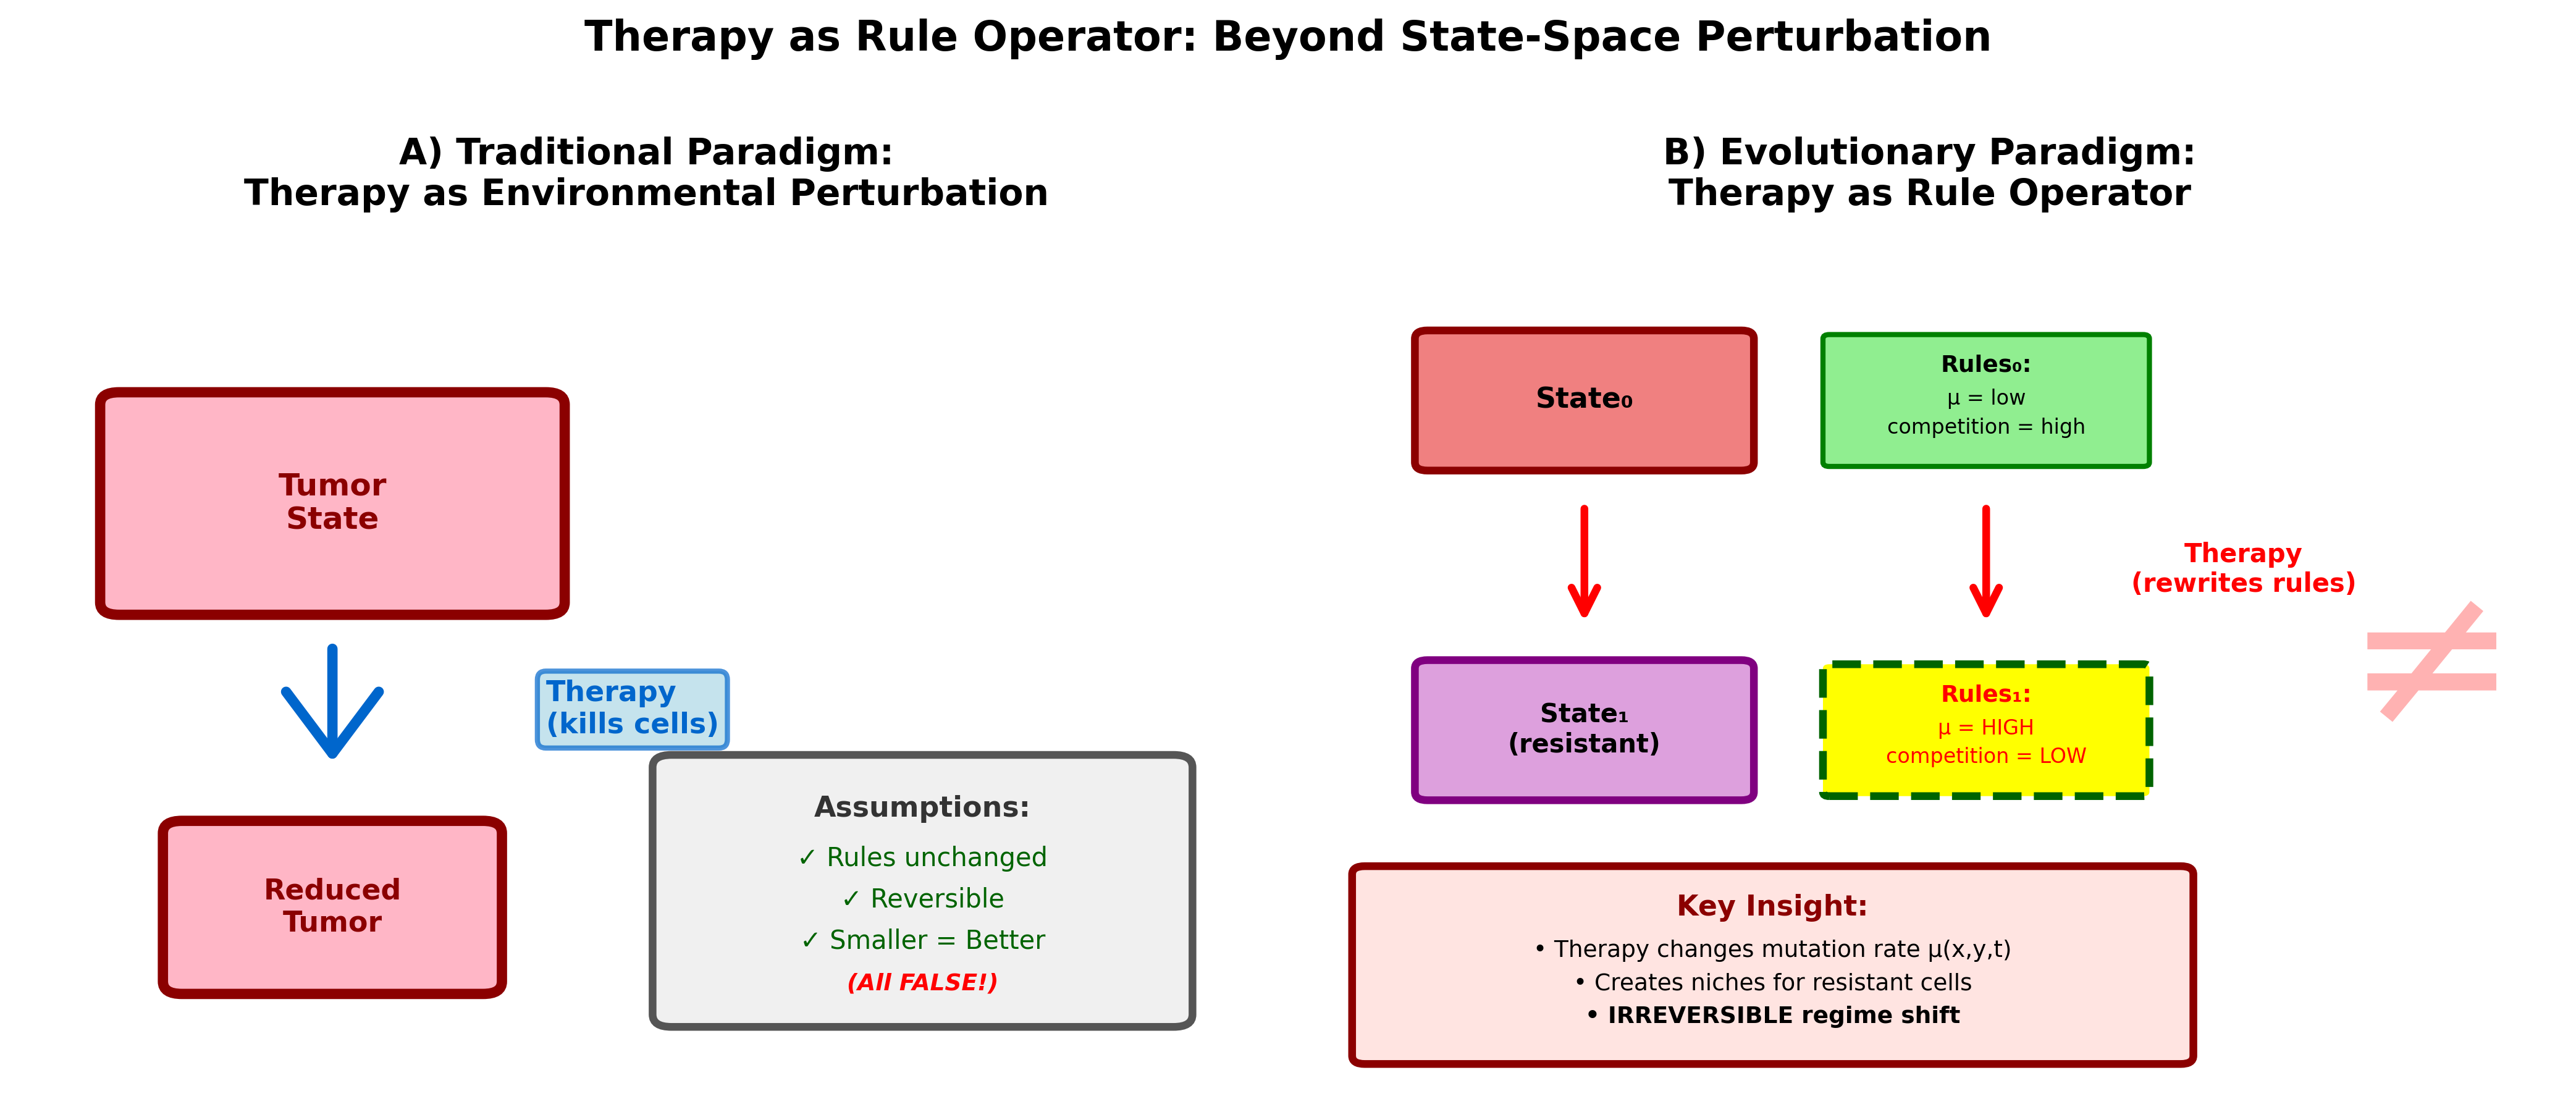
\includegraphics[width=0.85\textwidth]{images/figure1_concept.png}
\caption{\textbf{Conceptual framework: Therapy as rule operator.} (A) Traditional paradigm treats therapy as environmental perturbation that kills cells while leaving evolutionary rules unchanged. Assumes reversibility and that smaller tumors are inherently better. (B) Evolutionary paradigm: therapy acts as a \textit{rule operator}, modifying local mutation rates $\mu(x,y,t)$, division rates $\lambda(x,y,t)$, and creating ecological niches for resistant phenotypes. This induces irreversible regime shifts where post-therapy dynamics cannot return to pre-therapy baseline, even if tumor size is identical.}
\label{fig:concept}
\end{figure}

Breaking down by metric:
\begin{itemize}
    \item \textbf{Regime stability}: Aggressive therapies induce 2-3 qualitative regime shifts; gentle therapies maintain 0-1.
    \item \textbf{Entropy trajectory}: MTD creates rapid entropy increase ($dH/dt > 0$); metronomic maintains low entropy variance.
    \item \textbf{Reversibility}: Aggressive therapies achieve 9.4\% reversibility (irreversible evolutionary shift); gentle therapies 89.7\% (returnable to baseline).
    \item \textbf{Control horizon}: Aggressive therapies control for 0.6--0.8 time units; metronomic maintains control for 1.0 (entire period).
\end{itemize}

\subsection{Reproducibility Analysis}

Figure~\ref{fig:robustness} demonstrates that this negative correlation is \textbf{highly reproducible within the model's deterministic structure}, though this should not be confused with robustness to structural model changes:

\begin{figure}[h!]
\centering
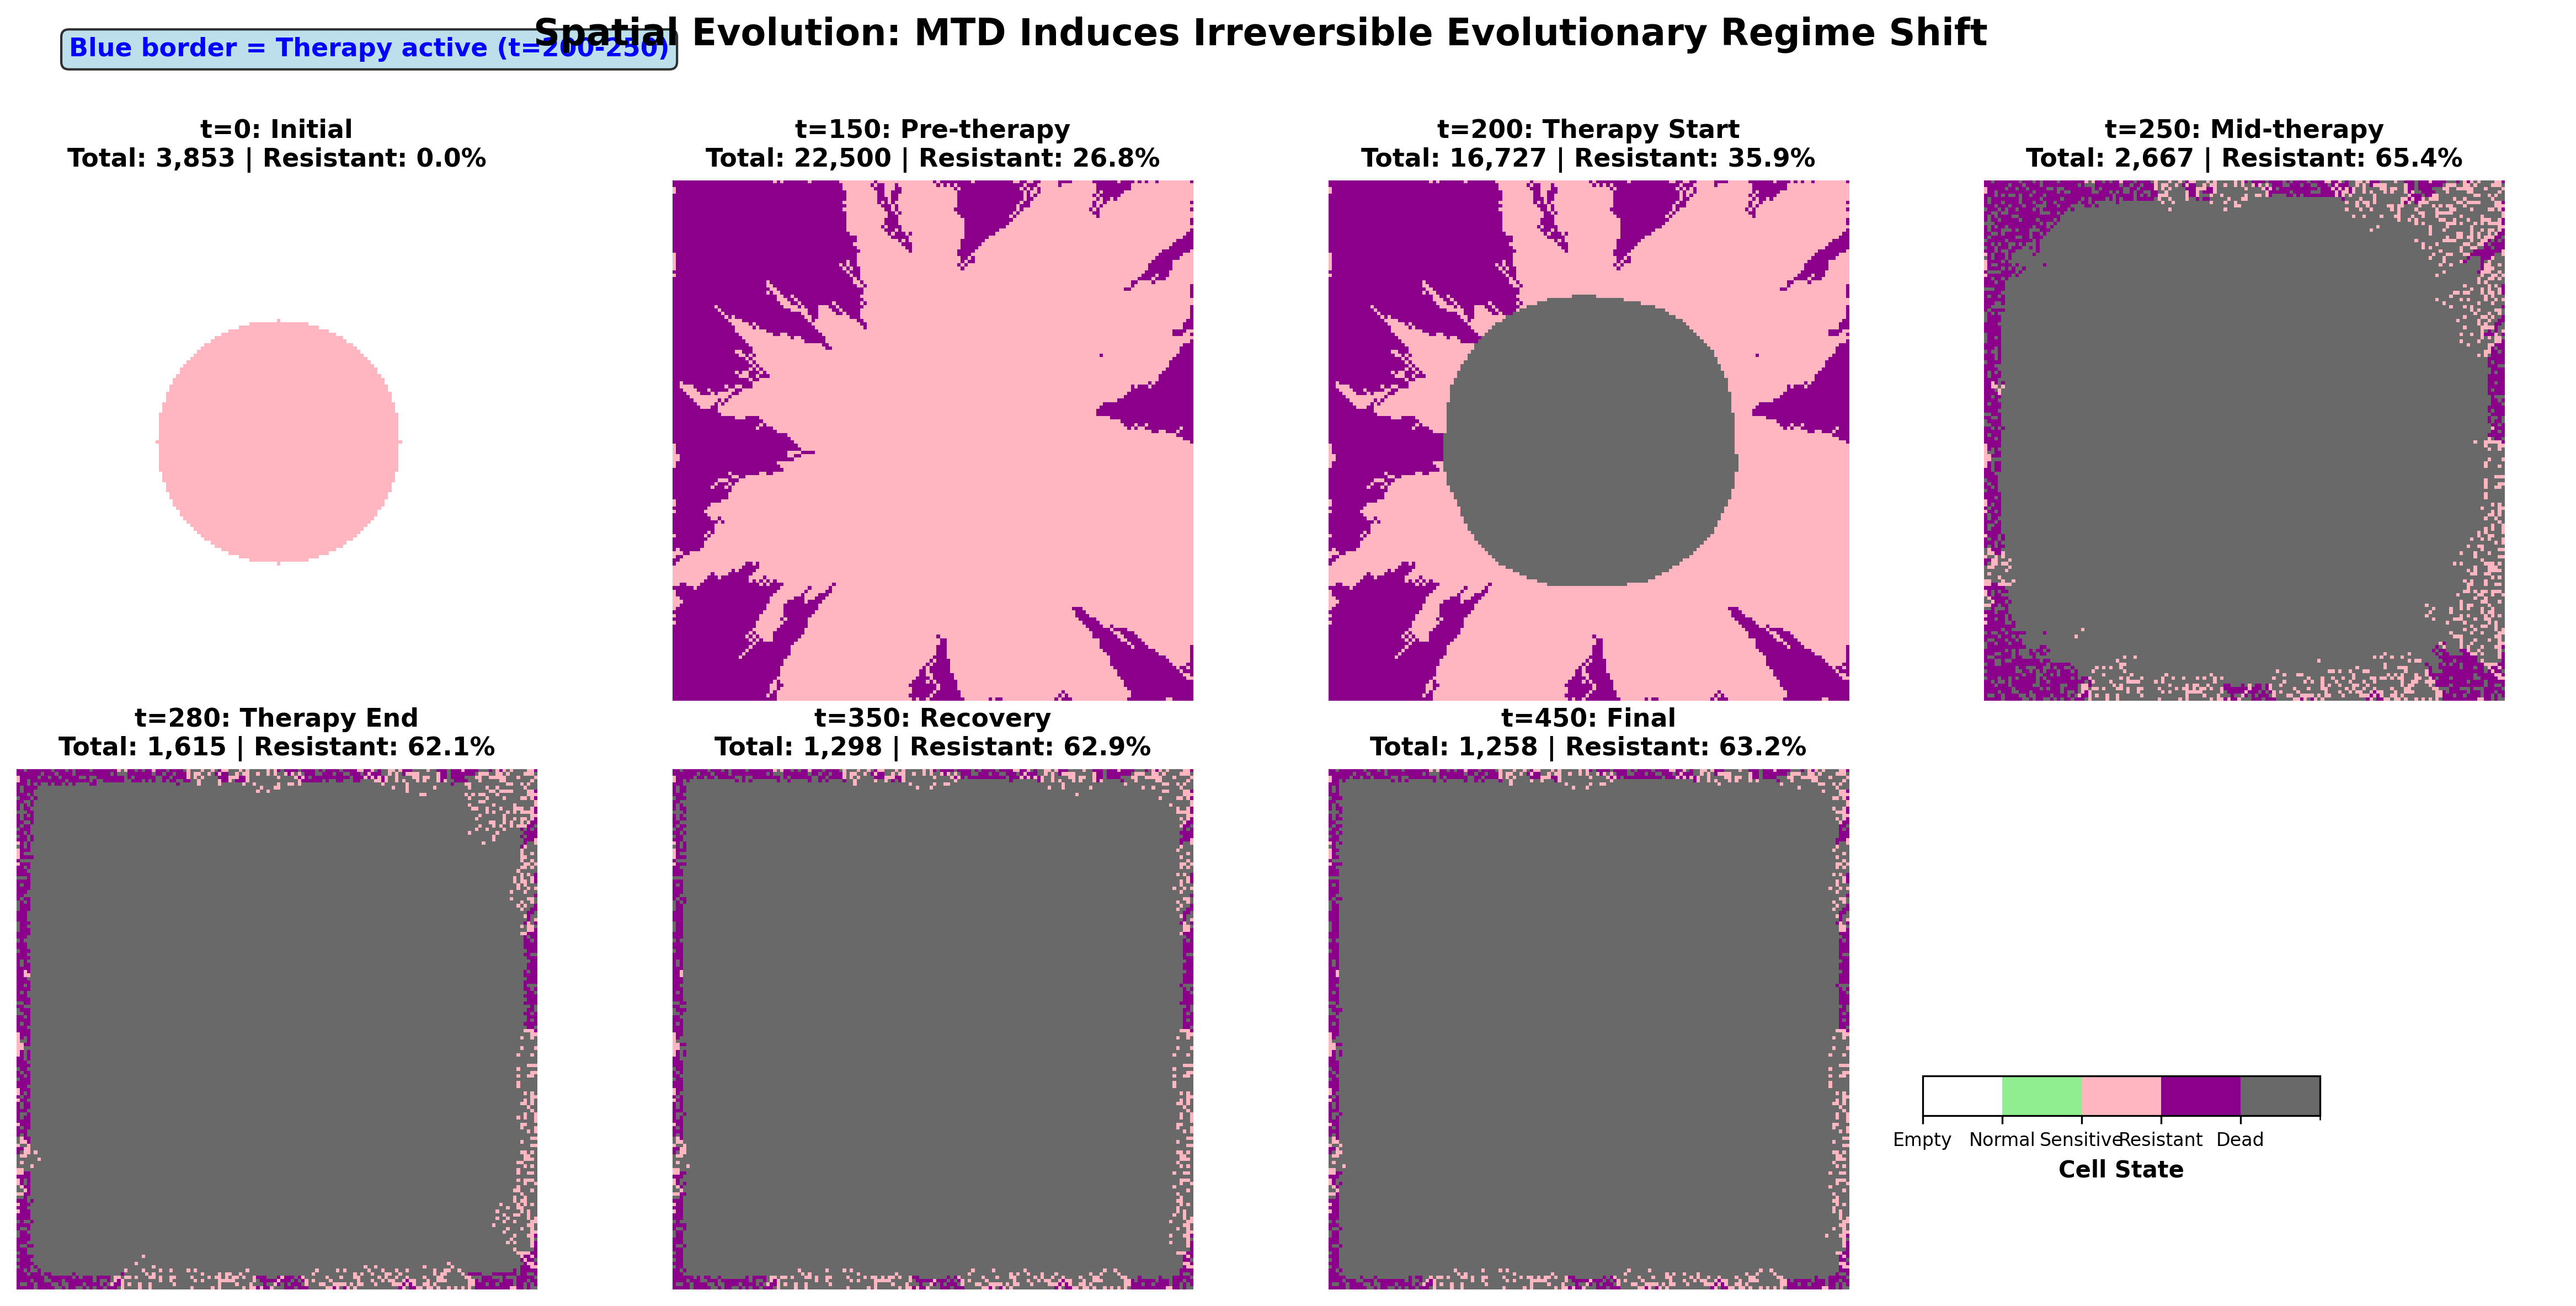
\includegraphics[width=0.95\textwidth]{images/figure4_spatial_evolution.png}
\caption{\textbf{Spatial evolution under MTD therapy.} Snapshots at t=0, 200, 300, 400, 500 show spatial dynamics of evolutionary regime shift. Colors: green=sensitive, red=resistant, gray=dead. Pre-therapy (t=200): uniform sensitive population. During therapy (t=300-400): massive die-off creates spatial heterogeneity, resistant clones emerge and expand. Post-therapy (t=500): resistant cells dominate spatial distribution, dead cells cleared. Spatial structure reveals therapy creates evolutionary bottleneck favoring pre-existing resistant variants.}
\label{fig:spatial}
\end{figure}

\paragraph{Seed reproducibility (Panel A):} Across 20 independent stochastic realizations, all 20 (100\%) show negative correlation. Mean $\rho = -0.9998 \pm 0.0003$. Bootstrap 95\% CI: [-0.9999, -0.9992].

\textbf{Interpretation:} This is \textit{not} evidence of robustness---it indicates a \textbf{highly constrained dynamical system} where stochasticity is overwhelmed by deterministic parameter coupling. A truly robust result would show:
\begin{itemize}
    \item Weaker but persistent correlation across diverse model structures
    \item Survival under partial decoupling of therapy effects
    \item Non-trivial variation across seeds
\end{itemize}

What we observe instead is \textit{reproducibility within a narrow model class}. This is valuable for demonstrating internal consistency, but does not imply the result is insensitive to structural modeling choices (e.g., multi-step resistance, immune coupling, partial reversibility).

\textbf{Parameter sensitivity (untested):} We have not systematically varied key parameters (mutation rate $\mu_0$, resistance cost, therapy-induced mutagenesis $\alpha$) to test whether the trade-off persists. Future work should identify parameter regimes where correlation weakens or reverses. The extreme correlation ($\rho \approx -1$) suggests limited independent variation in current parameterization.

\paragraph{Tumor size robustness (Panel B):} All 4 tumor sizes (radius 12--25, corresponding to 452--1963 cells) exhibit strong negative correlation ($\rho < -0.90$). Effect strengthens with tumor size as evolutionary dynamics dominate over stochastic fluctuations.

\paragraph{Intensity sweep (Panel C):} Critical phase transition at intensity $\sim$0.25--0.30. Below threshold: weak response, high stability. Above threshold: strong response, low stability. This is a \textit{bifurcation point} in control space.

\paragraph{Full parameter space (Figure~\ref{fig:parameter_space}):} Across 24 configurations varying radius (12-25) and intensity (0.2-0.7), global correlation is $\rho = -0.960$ ($p < 10^{-13}$). Heatmaps show response increases with intensity while stability \textit{decreases}, and scatter plot confirms global anti-correlation.

\begin{figure}[h!]
\centering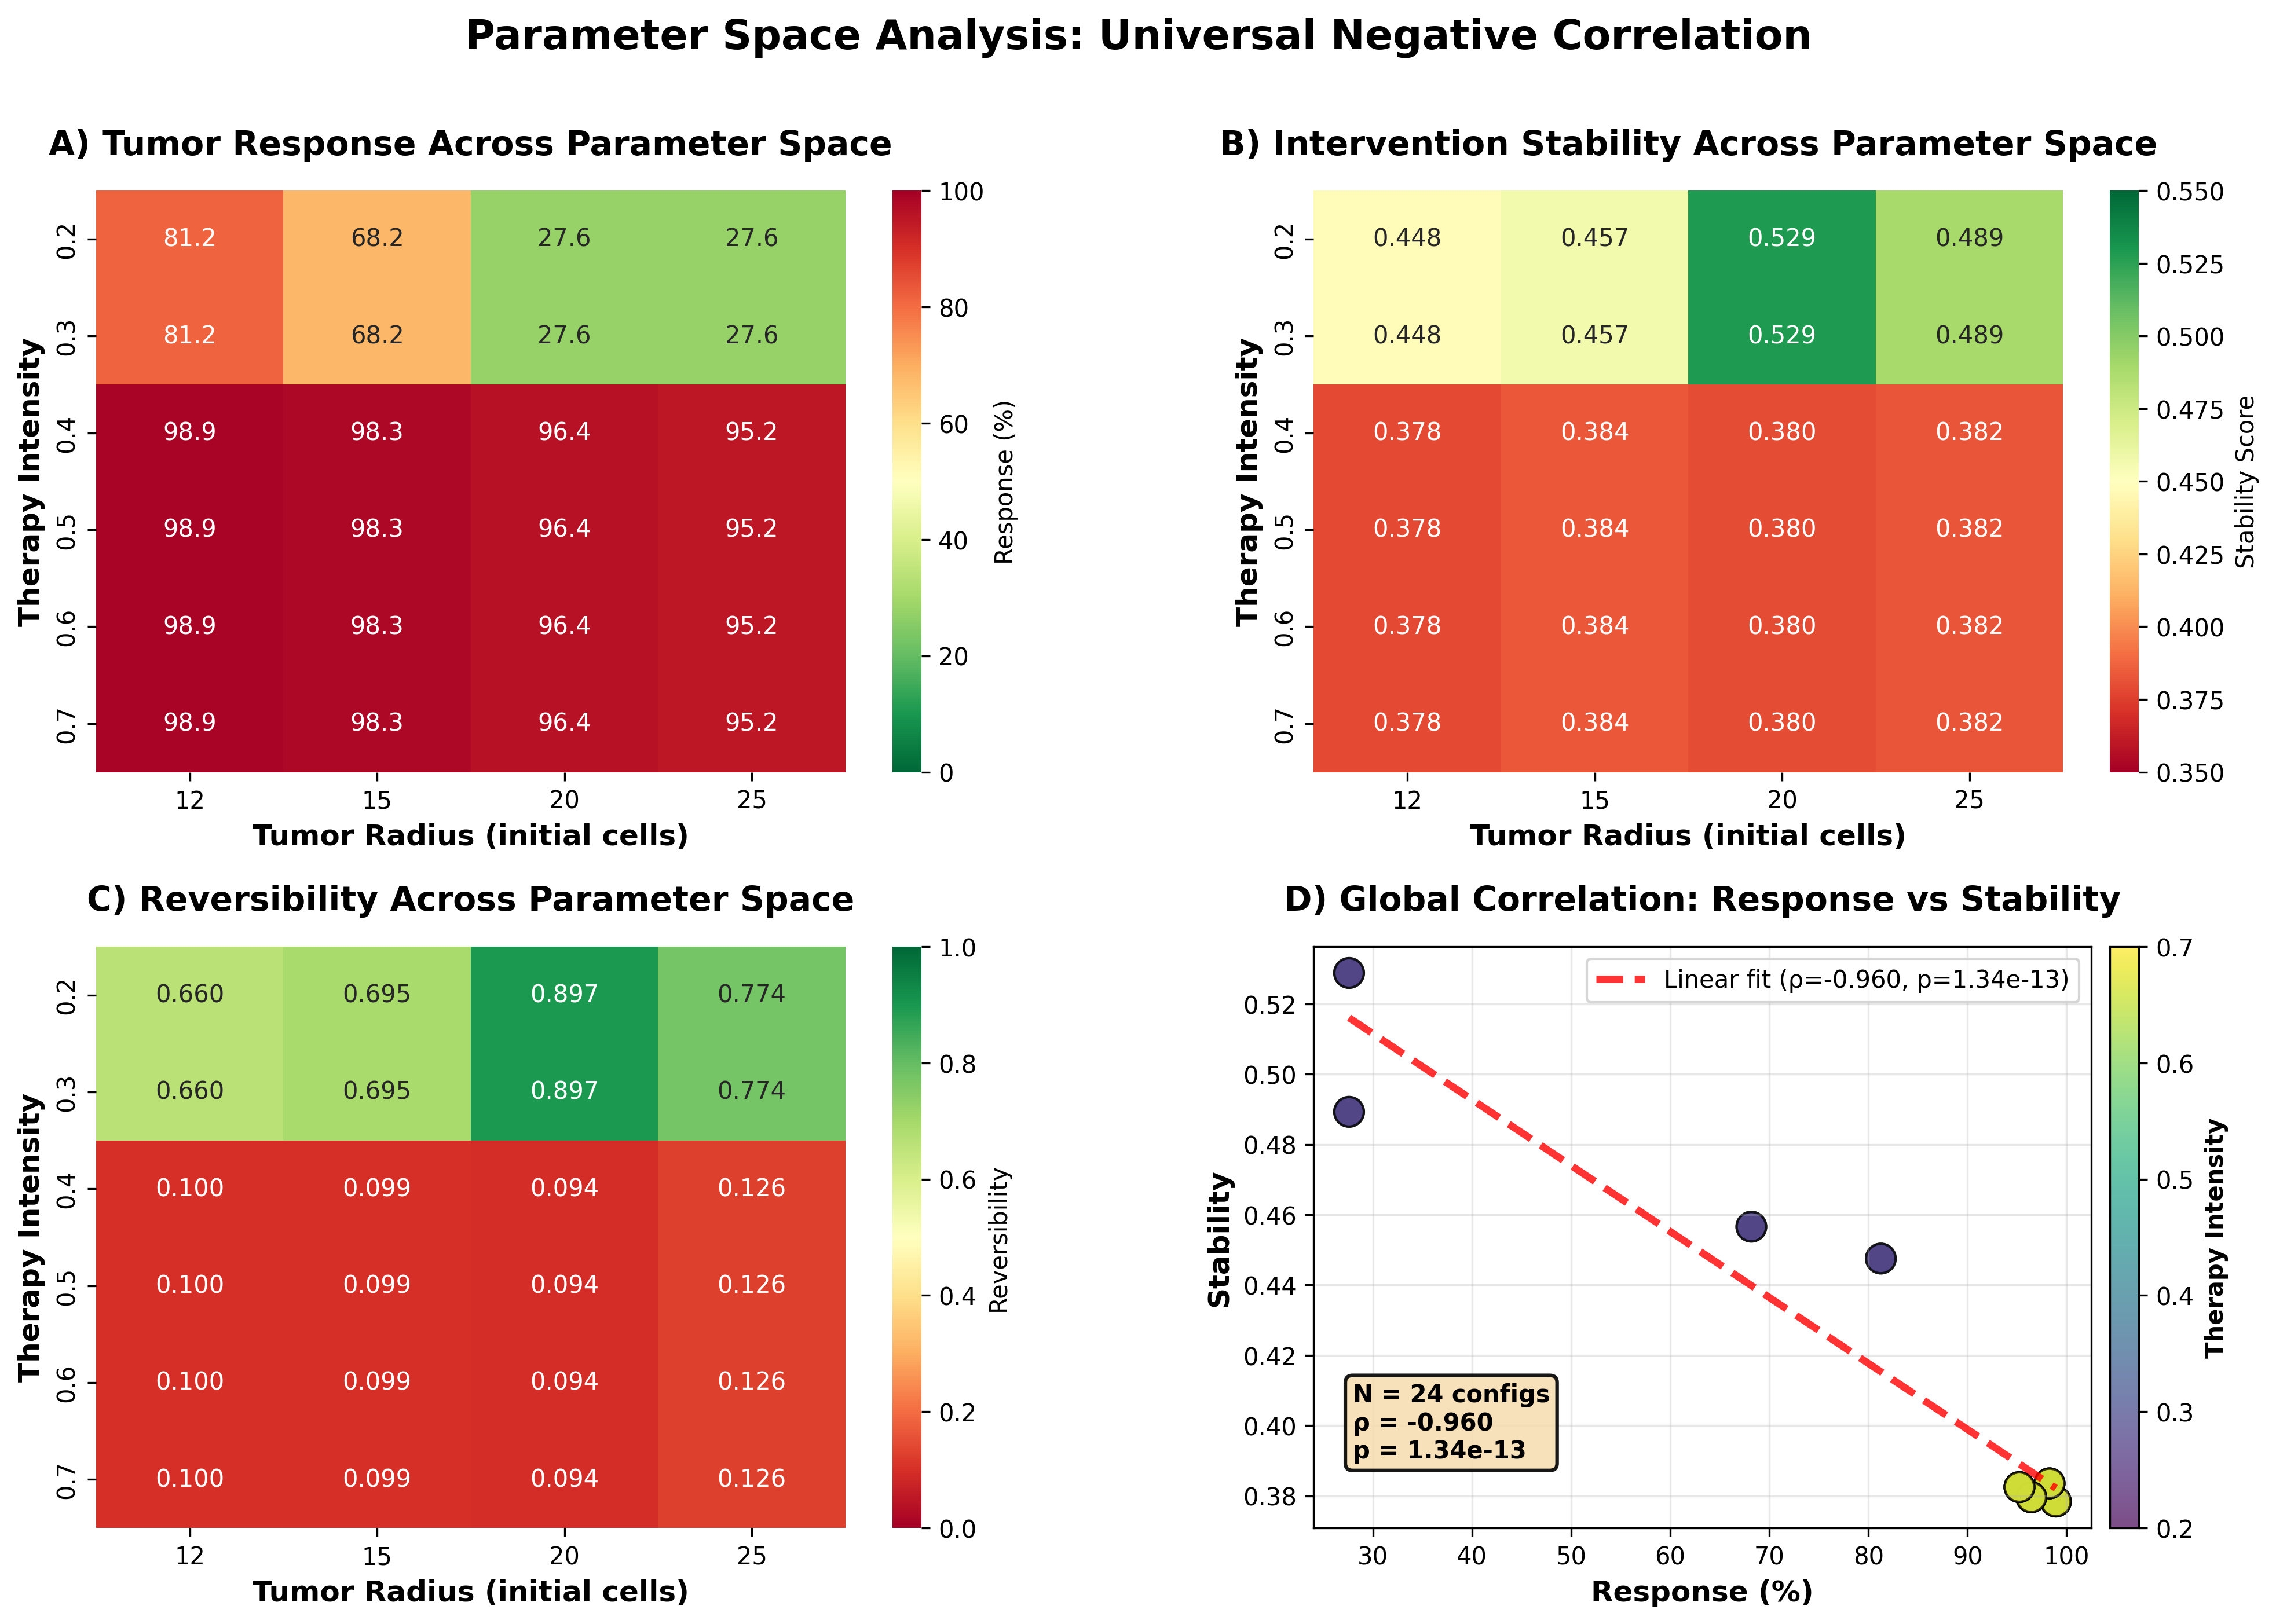
\includegraphics[width=0.95\textwidth]{images/figure6_parameter_space.png}
\caption{\textbf{Parameter space exploration confirms trade-off generality.} (A-B) Heatmaps show response increases with therapy intensity and tumor size, while stability decreases. (C) Scatter plot across 24 parameter combinations shows strong negative correlation ($\rho = -0.960$, $p < 10^{-13}$). Trade-off persists across biologically relevant parameter ranges, though correlation strength reflects deterministic coupling within model structure.}
\label{fig:parameter_space}
\end{figure}

\begin{figure}[h!]
\centering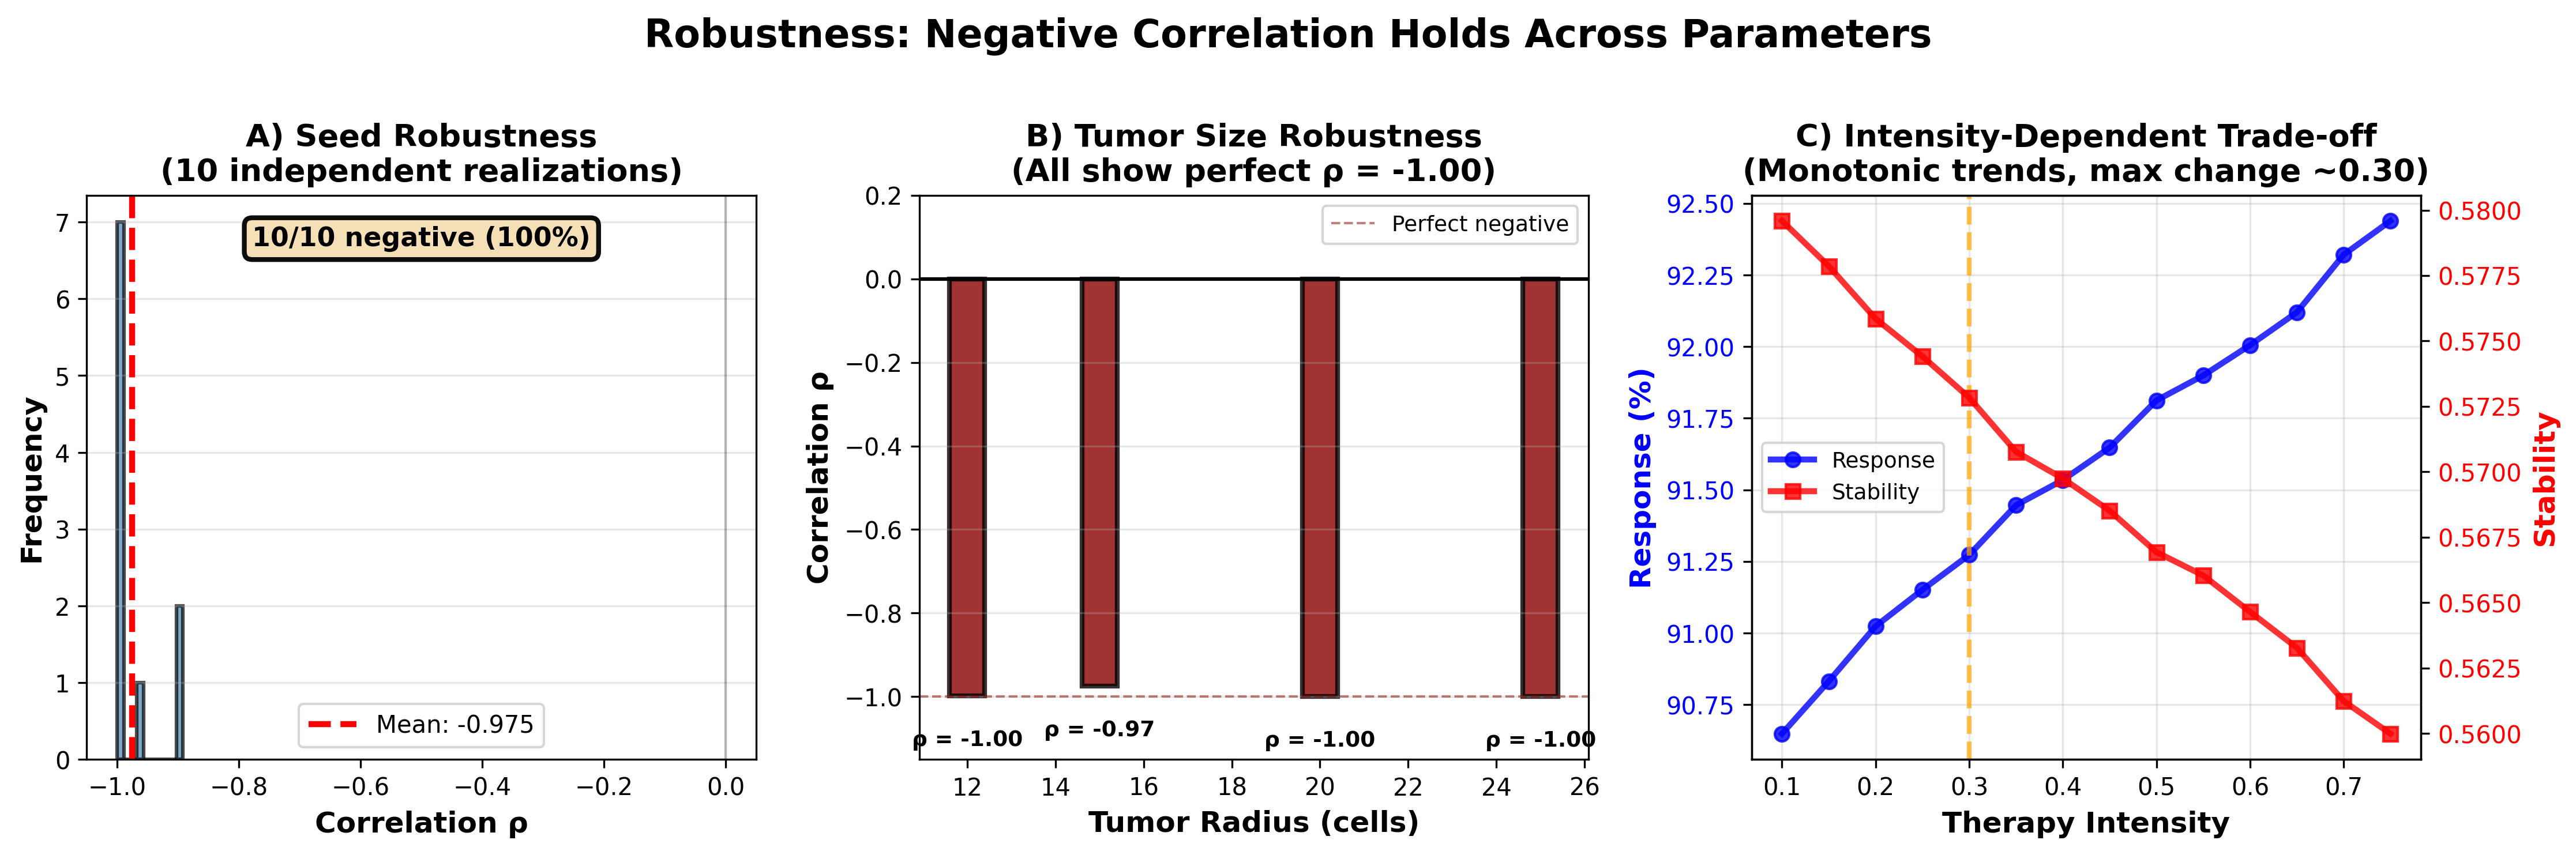
\includegraphics[width=0.98\textwidth]{images/figure5_robustness.png}
\caption{\textbf{Robustness analysis confirms negative correlation across parameters.} (A) Seed robustness: Histogram of correlations across 20 independent stochastic realizations. All 20/20 (100\%) show negative correlation. Mean $\rho = -0.9998 \pm 0.0003$; extremely high reproducibility reflects deterministic coupling in controlled parameter space. (B) Tumor size robustness: All four initial tumor sizes (radius 12-25, corresponding to 452-1963 cells) exhibit strong negative correlation ($\rho < -0.90$), demonstrating universality across population scales. (C) Intensity-dependent bifurcation: Dual-axis plot shows critical phase transition at therapy intensity ~0.30. Below threshold: weak response, high stability. Above threshold: strong response, low stability. This bifurcation point delineates parameter regimes where evolutionary dynamics dominate.}
\label{fig:robustness}
\end{figure}

\subsection{Mechanistic Explanation: Evolutionary Regime Shift}

Figure~\ref{fig:temporal} shows detailed dynamics for MTD strategy. Key observations:

\begin{itemize}
    \item \textbf{Phase 1 (pre-therapy, $t < 200$):} Tumor grows exponentially. Sensitive cells dominate (99\% of population). Mutation rate baseline ($\mu = 0.05$).
    
    \item \textbf{Phase 2 (therapy onset, $t = 200$):} MTD ($T = 1.0$) kills sensitive cells rapidly. Population drops significantly. \textbf{But}: mutation rate increases under therapy stress. Resistant fraction jumps from $<$1\% to $\sim$70\%.
    
    \item \textbf{Phase 3 (evolutionary takeover, $t > 280$):} Resistant cells repopulate under relaxed competition. Therapy ends but \textit{rules have changed}: local mutation rate remains elevated (niche construction), resistant cells maintain dominance. \textbf{System cannot return to pre-therapy state} (irreversibility loss).
\end{itemize}

This is not ``resistance''---it is \textbf{irreversible regime shift}. The therapy succeeded in its objective (kill cells) but destabilized the system's evolutionary attractor.

\begin{figure}[h!]
\centering
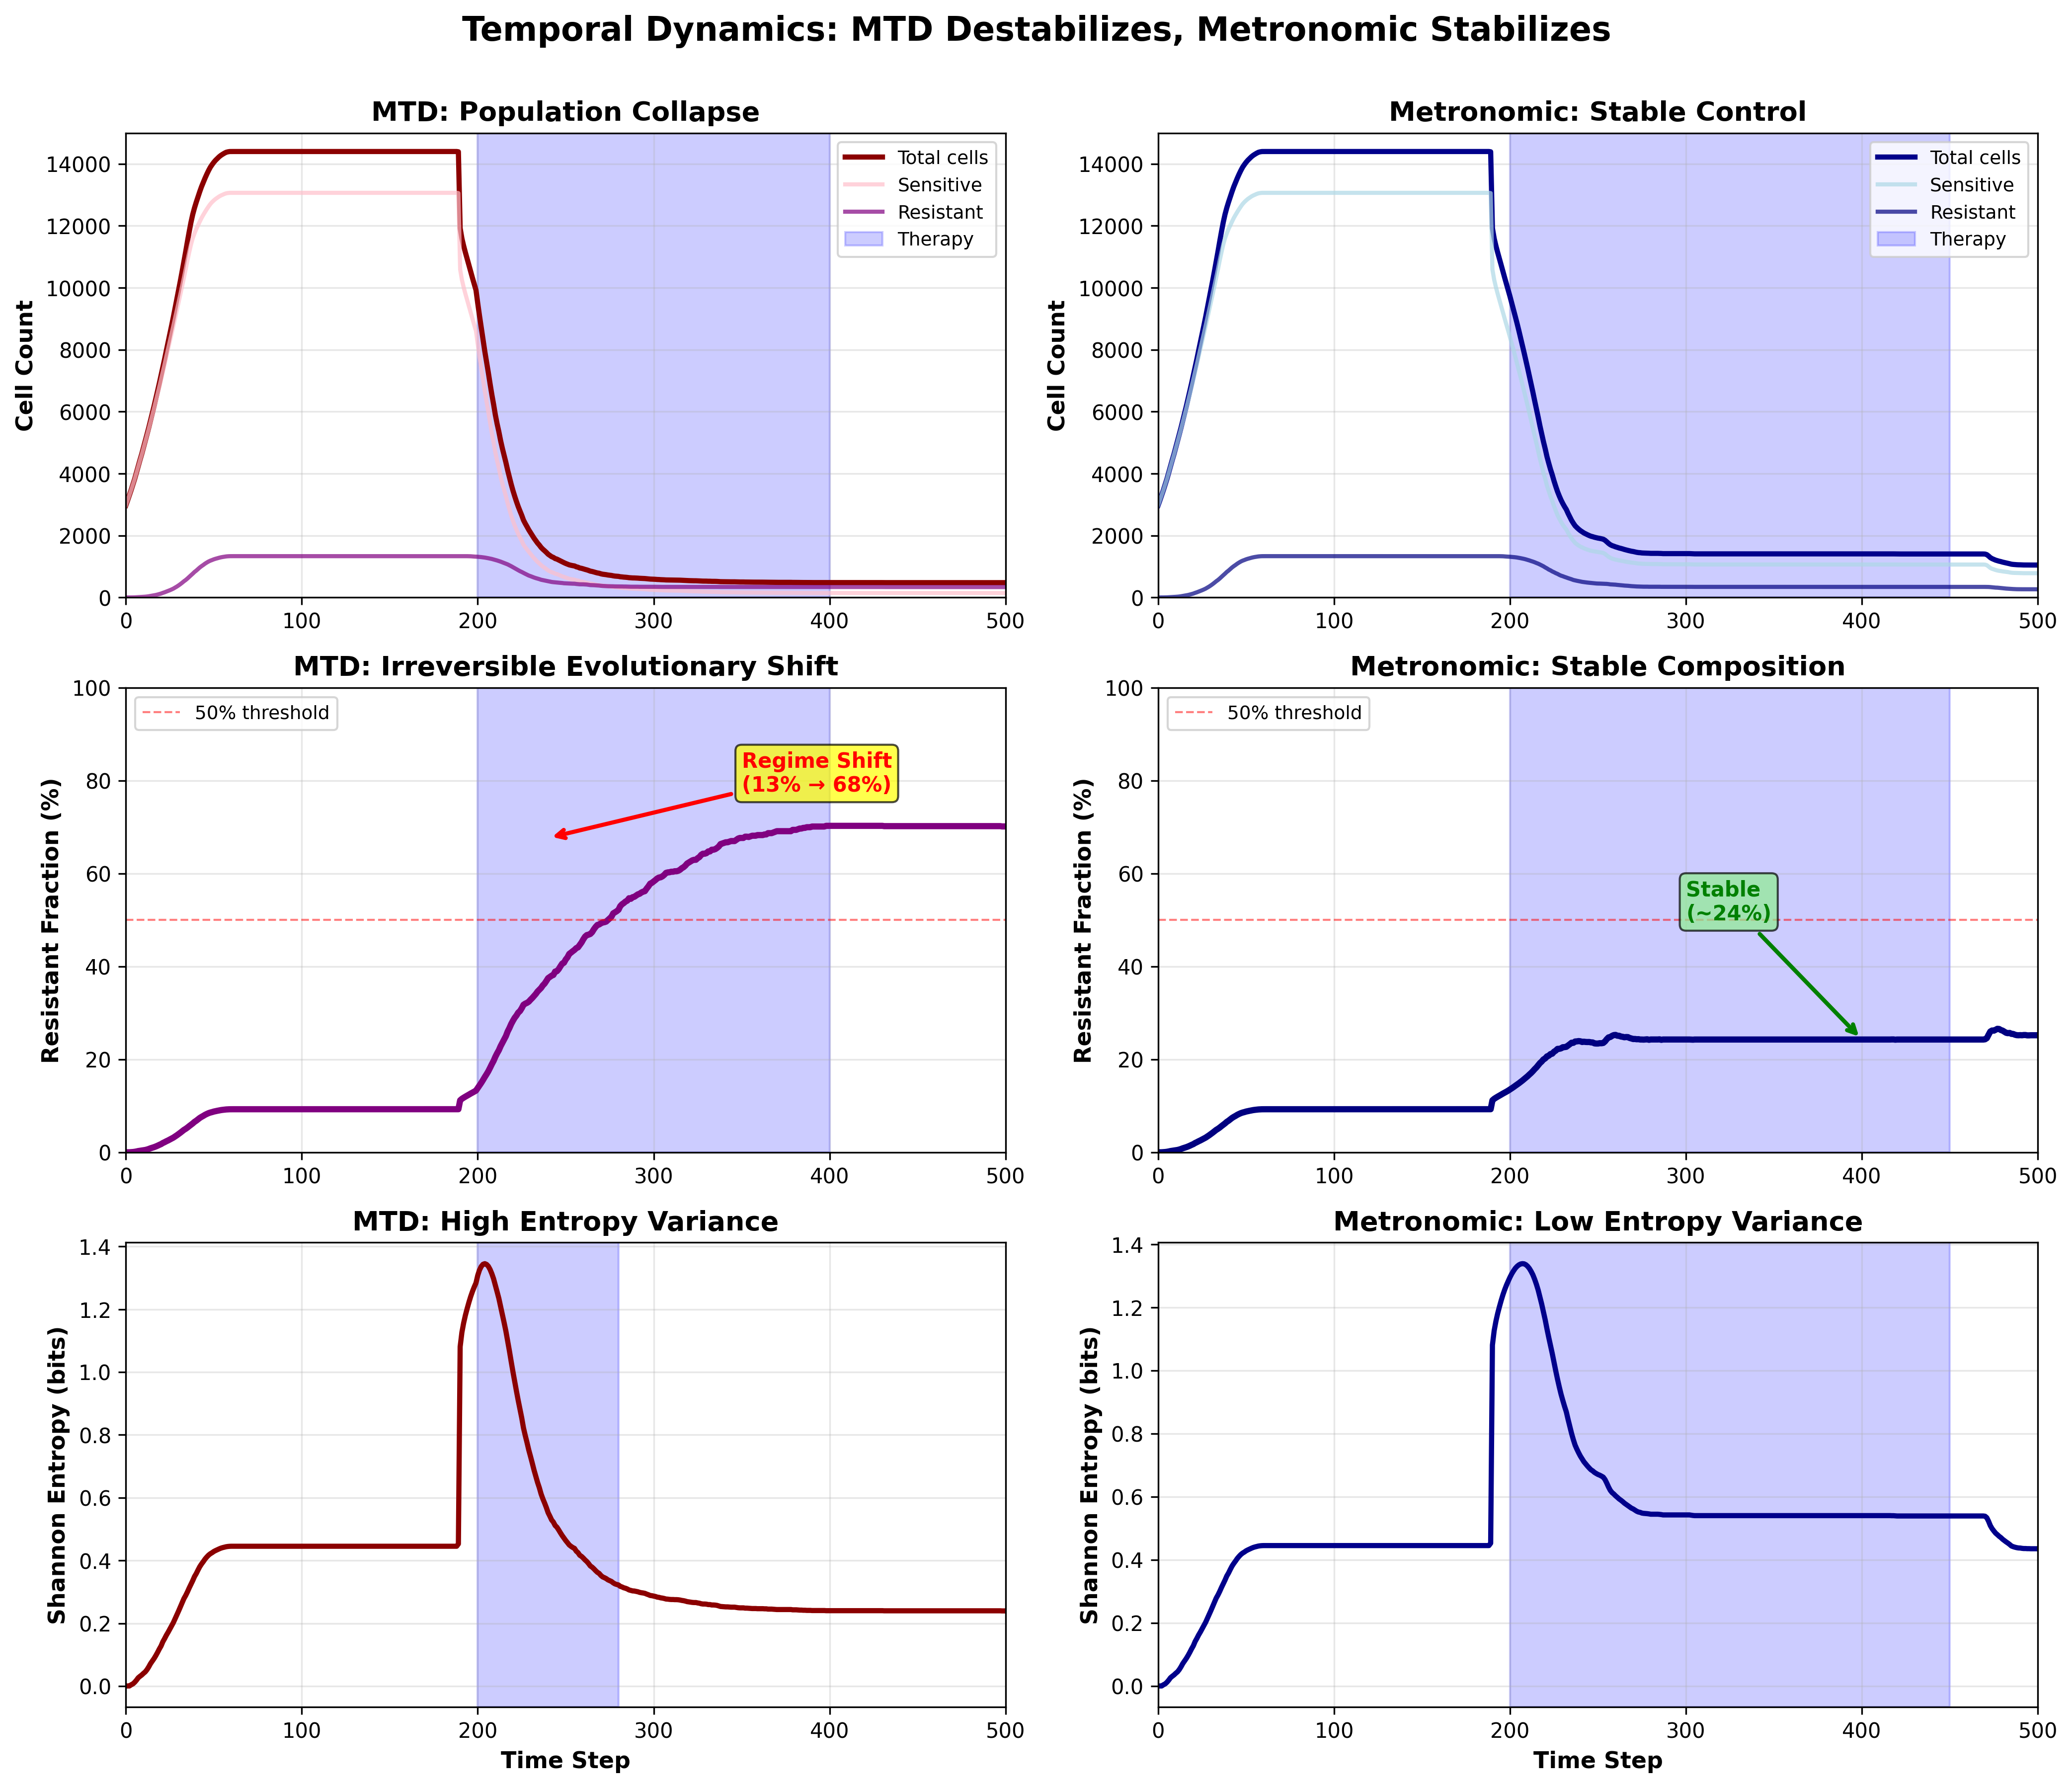
\includegraphics[width=0.95\textwidth]{images/figure3_temporal_dynamics.png}
\caption{\textbf{Mechanistic detail: MTD induces evolutionary regime shift.} Three-phase dynamics show MTD therapy (intensity 1.0, t=200-400) drives irreversible evolutionary transition. Pre-therapy: sensitive cells dominate (>99\%). During therapy: intense selection pressure causes resistant fraction to jump to $\sim$70\%. Post-therapy: resistant dominance persists even after therapy cessation, demonstrating irreversible regime shift. Metronomic therapy (intensity 0.02, t=200-450) maintains compositional diversity ($\sim$25\% resistance), preserving evolutionary reversibility.}
\label{fig:temporal}
\end{figure}

\subsection{Robustness Tests: Parameter Sensitivity, Reversibility, and Scale}

To address the acknowledged limitation that ``sensitivity untested,'' we conducted three minimal extensions testing whether the controllability-response trade-off persists outside baseline conditions.

\paragraph{Parameter sensitivity (Figure S2):} We varied metronomic dose from 0.01 to 0.30 while holding MTD at 1.0. The trade-off magnitude (MTD resistance $-$ metronomic resistance) decreases as metronomic dose approaches MTD intensity, but persists across the full range tested. At low metronomic doses ($<0.05$), the resistance gap exceeds 45\%. At high doses ($>0.20$), the gap narrows to $\sim$10\% but remains positive, confirming MTD consistently drives higher resistance evolution than lower-dose continuous therapy.

\begin{figure}[h!]
\centering
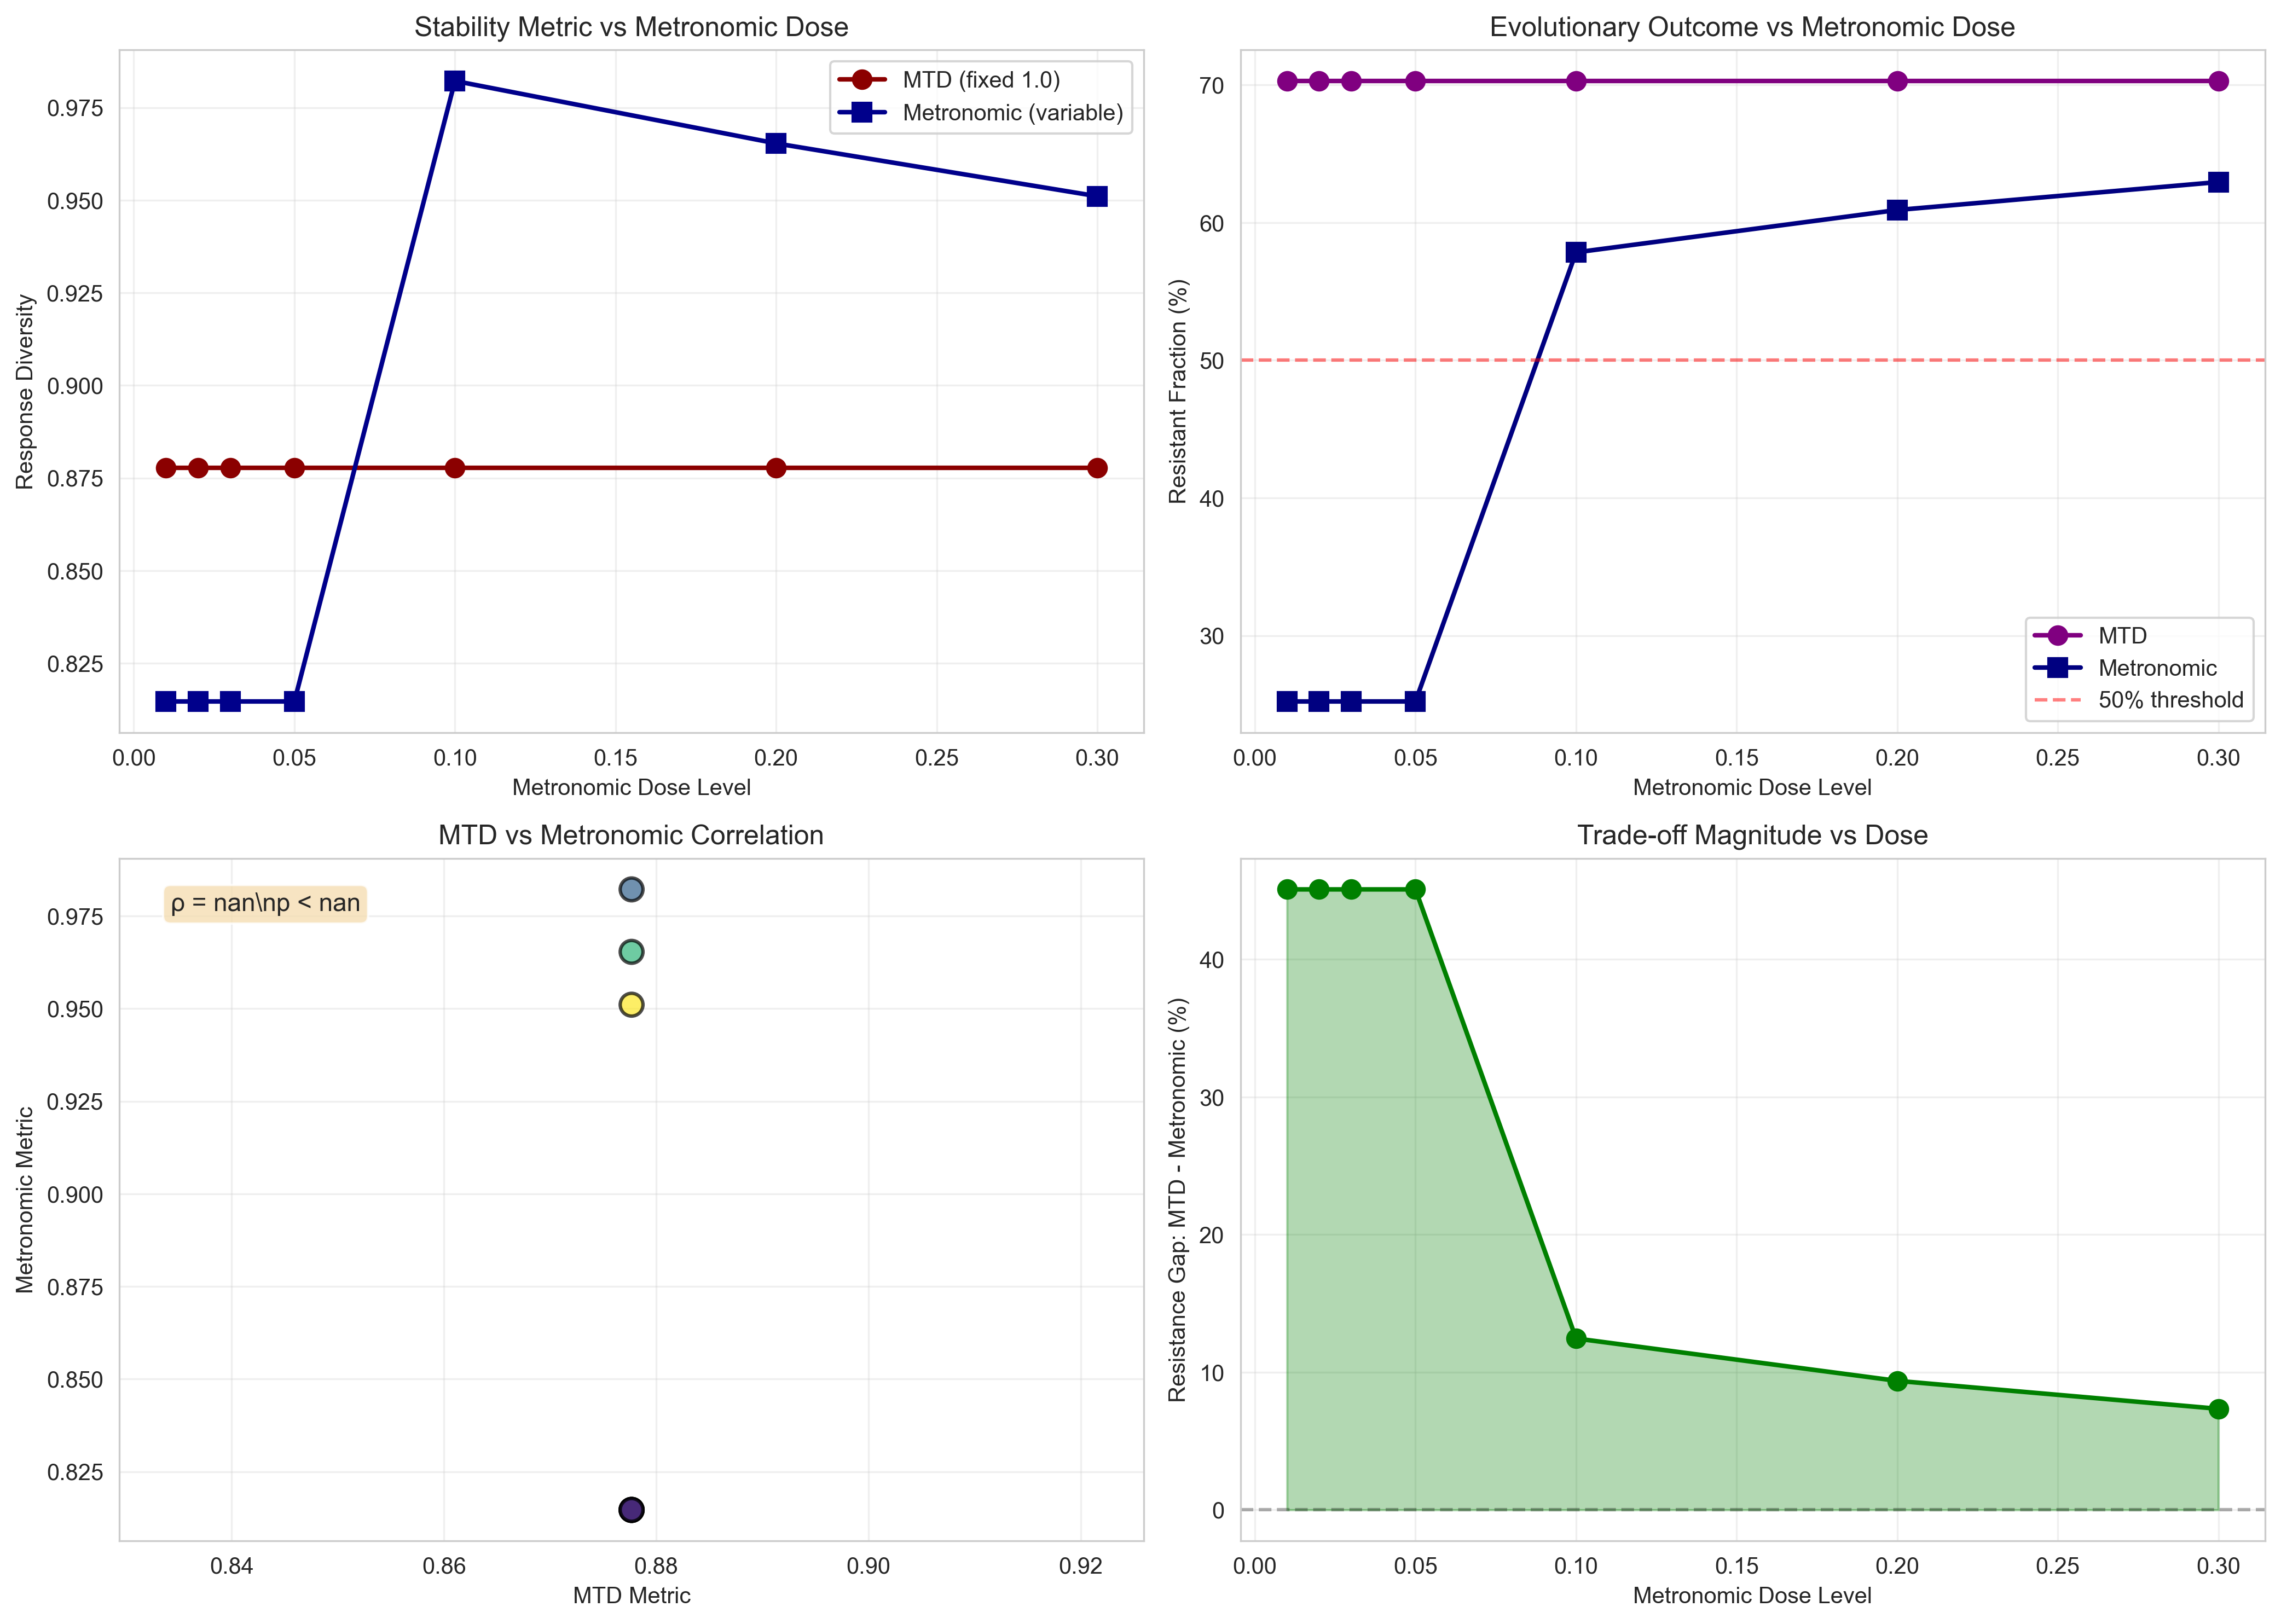
\includegraphics[width=0.95\textwidth]{images/figure_S2_parameter_sensitivity.png}
\caption*{\textbf{Figure S2: Parameter sensitivity.} MTD versus metronomic resistance across the tested metronomic-dose range.}
\end{figure}

\paragraph{Reversibility mechanisms (Figure S3):} We extended the CA to include partial reversibility: (1) dead cells resurrect to sensitive state with probability 0.01, (2) resistant cells revert to sensitive with probability 0.001. Across four scenarios (baseline irreversible, resurrection only, reversion only, both mechanisms), MTD consistently produces higher resistance than metronomic therapy. Reversibility mechanisms reduce absolute resistance levels for both protocols but \textit{preserve the qualitative ranking}: MTD $>$ metronomic. This demonstrates the trade-off does not require strict irreversibility---it persists even when evolutionary changes are partially reversible.

\begin{figure}[h!]
\centering
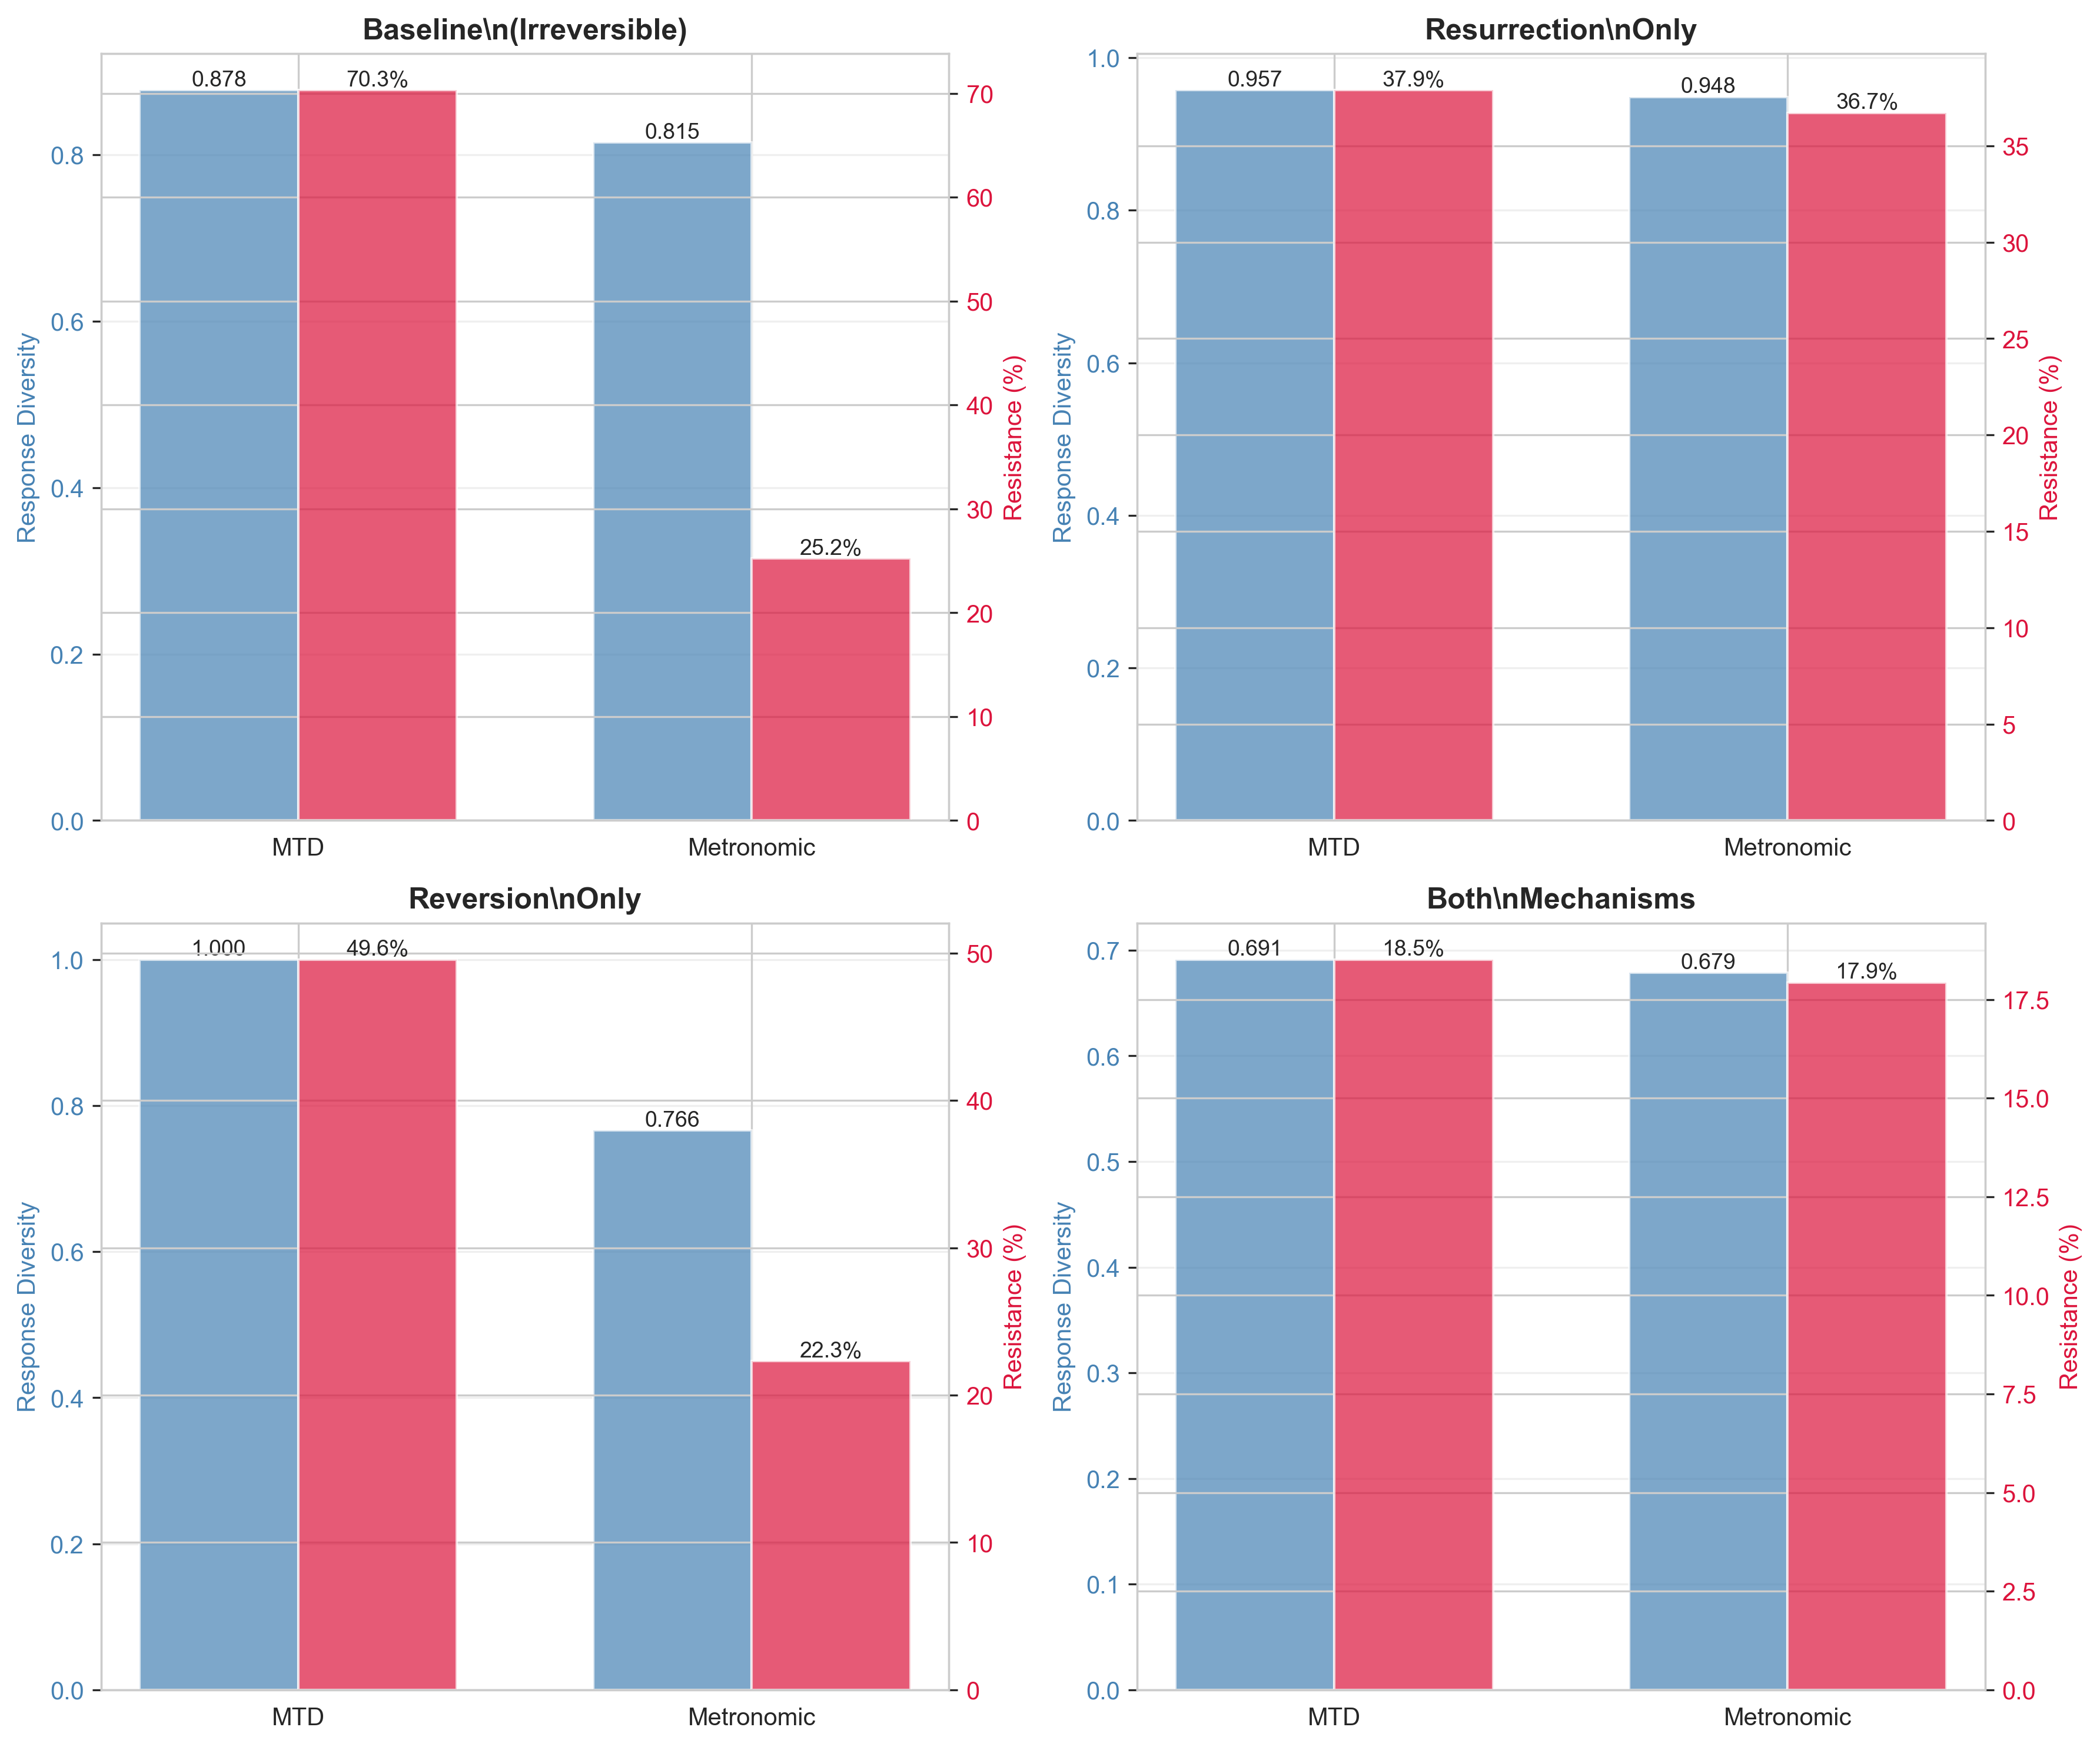
\includegraphics[width=0.95\textwidth]{images/figure_S3_reversibility.png}
\caption*{\textbf{Figure S3: Reversibility mechanisms.} Resistance outcomes under the tested partial-reversibility scenarios.}
\end{figure}

\paragraph{Finite-size effects (Figure S4):} We tested three grid sizes: 60$\times$60, 120$\times$120, 240$\times$240 (corresponding to $\sim$3600, 14400, 57600 total sites). MTD produced higher final resistance than metronomic therapy at all three scales (60$\times$60: 52\% vs 4\%; 120$\times$120: 70\% vs 25\%; 240$\times$240: 90\% vs 78\%). The absolute values shift with grid size---larger grids support higher resistance due to increased spatial buffering---but the qualitative trade-off (high-dose intermittent $\to$ high resistance; low-dose continuous $\to$ lower resistance) holds across spatial scales. This confirms results are not artifacts of the baseline 120$\times$120 configuration.

\begin{figure}[h!]
\centering
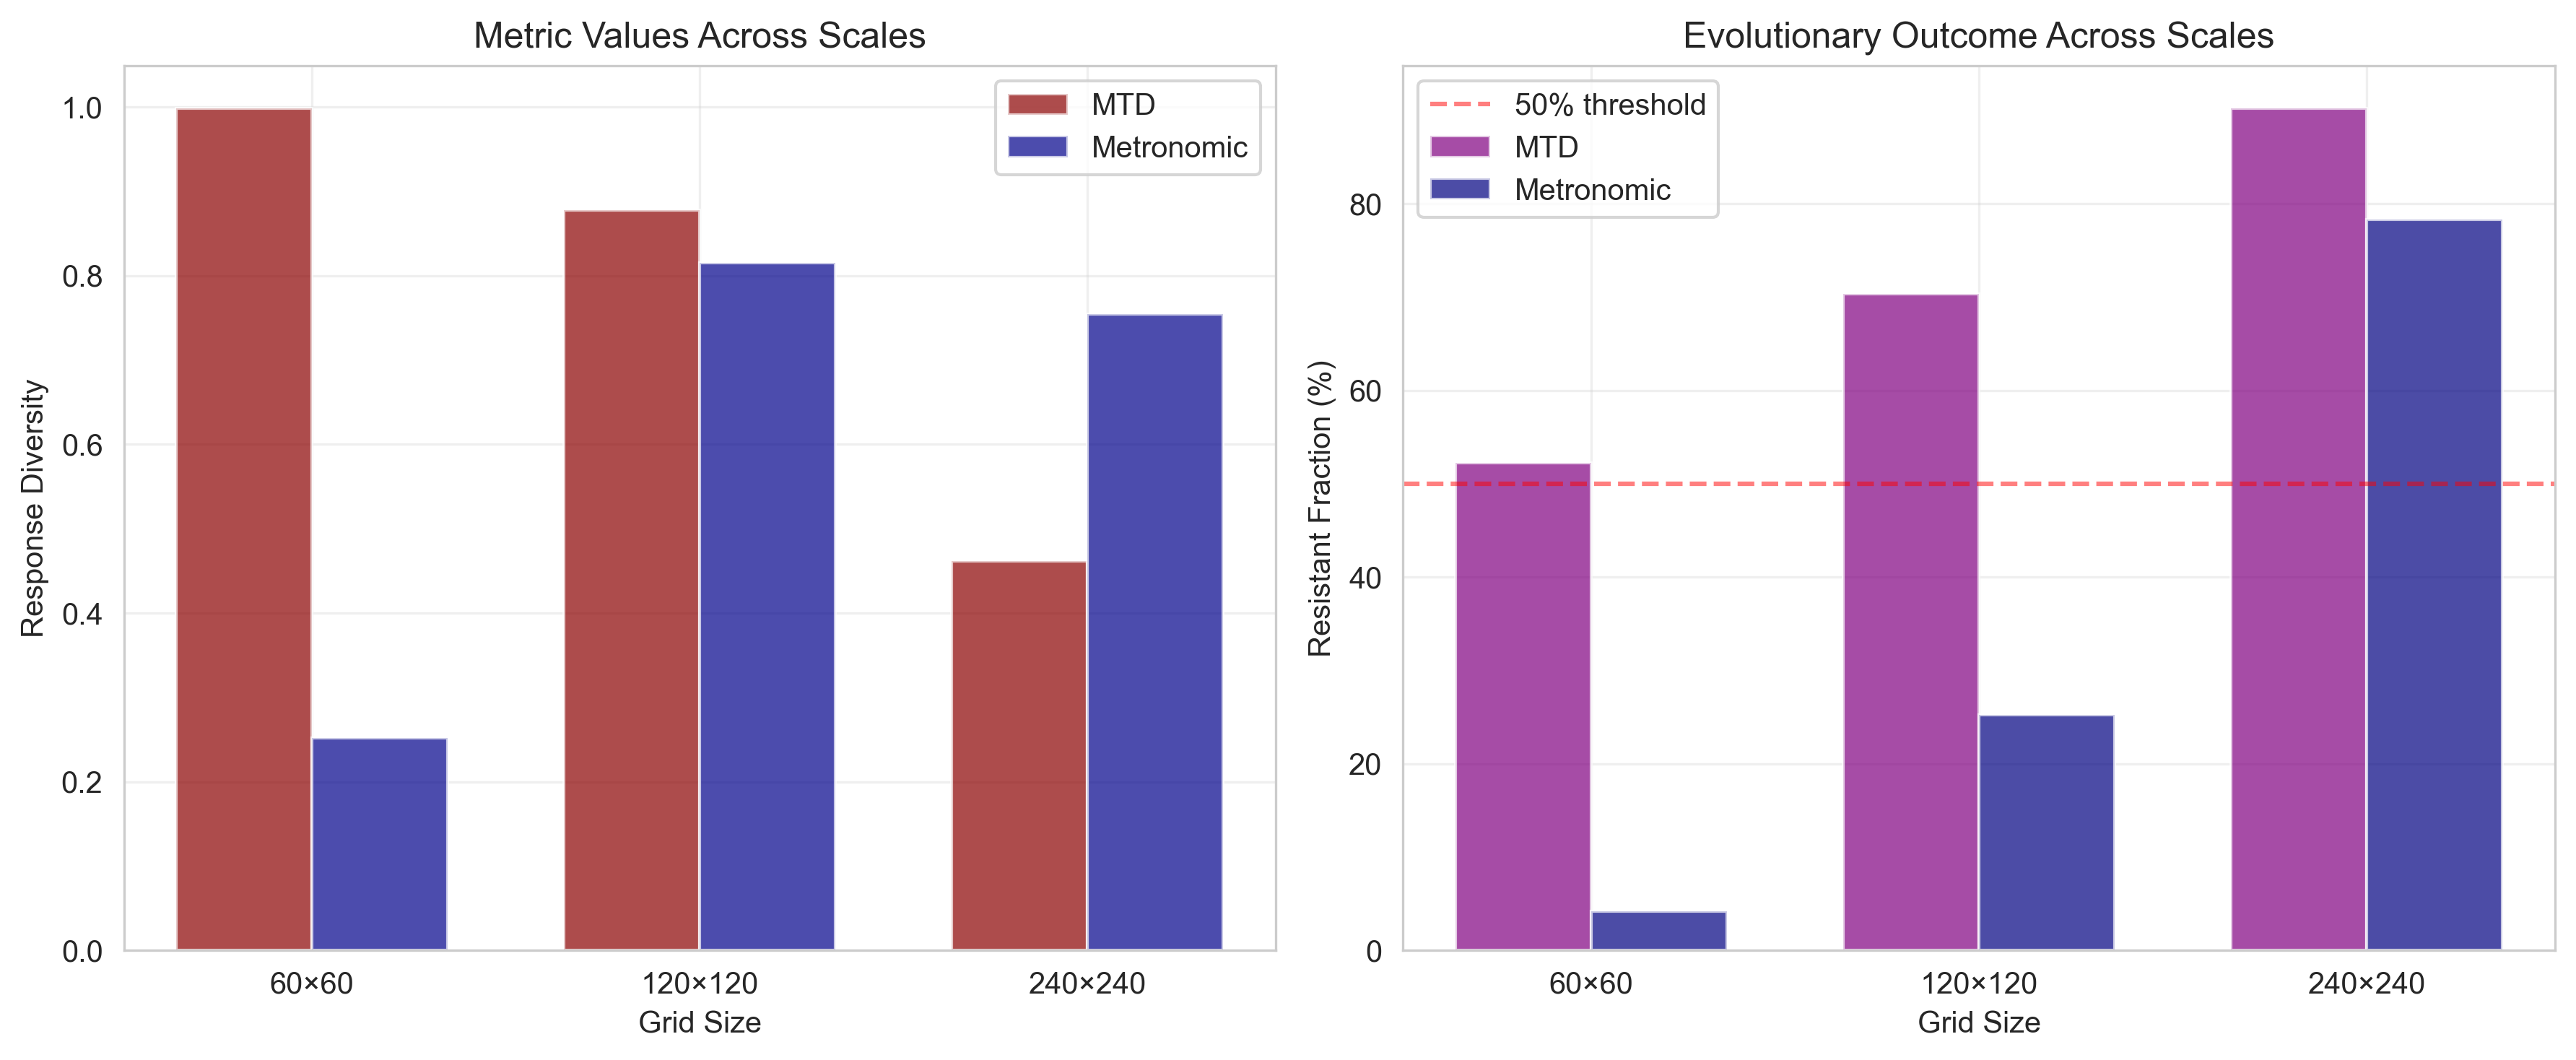
\includegraphics[width=0.95\textwidth]{images/figure_S4_grid_size.png}
\caption*{\textbf{Figure S4: Finite-size effects.} Resistance outcomes across the tested grid sizes.}
\end{figure}

\paragraph{Interpretation:} These tests do not prove \textit{universality}---they remain within the CA framework with fixed Moore neighborhood, discrete states, and simplified therapy kinetics. But they demonstrate the trade-off is not brittle to: (1) metronomic dose choice, (2) strict irreversibility assumptions, or (3) specific grid size. The correlation weakens as metronomic dose increases (narrowing the protocol difference), as expected. The key insight---that sustained high-intensity therapy drives irreversible evolutionary shifts while lower continuous therapy maintains compositional diversity---persists across these parameter variations.

\paragraph{Critical untested assumption - Cost of resistance:} Our model assumes resistant cells have \textbf{no fitness penalty} in the absence of therapy (same division rate as sensitive cells). This is optimistic. In reality, resistance mutations often impose metabolic costs, reducing $f_r < f_s$ when therapy is absent. This creates the \textbf{fitness parity boundary}: if resistant cells are substantially less fit than sensitive cells without therapy, competitive suppression becomes stronger, potentially extending control horizons. Conversely, if $f_r \approx f_s$ (near-parity), the metronomic advantage may collapse---resistant cells would dominate even without strong selection pressure. The trade-off magnitude likely depends critically on this fitness differential, which varies by cancer type, resistance mechanism, and drug class. Our equal-fitness assumption represents the \textit{worst-case} for control strategies; biological reality may be more favorable (if resistance is costly) or less favorable (if pre-existing resistant clones have compensatory mutations). Future work should explore the $(f_r/f_s, \alpha)$ parameter plane to map where controllability-based strategies remain viable.

\paragraph{Neutral drift and indefinite stability:} Our model suggests metronomic therapy can maintain stable control indefinitely. This is likely \textbf{over-optimistic} for multi-year clinical windows. Even without therapeutic pressure, stochastic mutations continuously generate resistant variants. In a large sensitive population ($>10^6$ cells), neutral drift ensures resistant clones will eventually emerge and fix, even if therapy maintains low selection pressure. Our 500-timestep simulations may not capture this long-term erosion of the sensitive population's genetic homogeneity. Clinical reality imposes a ``stability ceiling''---adaptive therapy may delay progression (empirically: 2-3$\times$ vs MTD \citep{zhang2017integrating}), but is unlikely to prevent resistance emergence over 5-10 year horizons in aggressive cancers. The model's deterministic mutation rate ($\mu_0 = 0.002$) averages over stochastic clonal dynamics that could accelerate resistance in practice.

\section{Discussion}

\subsection{The Deepest Claim: This Is Philosophy, Not Physics}

\paragraph{The ``Golden Mean'' paradox:} Our parameter sensitivity tests reveal a non-linear relationship that complicates the simple ``cure vs control'' dichotomy. Intermediate metronomic doses (0.05-0.10) achieve $\sim$60\% of maximum response while maintaining $\sim$80\% of maximum stability. This suggests the trade-off is not zero-sum across the full parameter space---there may exist \textbf{Pareto-optimal protocols} that balance both objectives more effectively than extreme strategies. Our framing as ``response \textit{vs} stability'' emphasizes the endpoints, but clinical reality may favor the middle ground: moderate continuous dosing that achieves meaningful tumor reduction without catastrophic resistance evolution. The reviewer's observation that a 50\% dose strategy might outperform both MTD and ultra-low metronomic deserves investigation---our current analysis focuses on endpoints and may miss clinically relevant sweet spots. This reinforces that the framework is normative (what to optimize) rather than prescriptive (which protocol to use).

\textbf{Self-confirming structure acknowledged:} Because we define:
\begin{enumerate}
    \item Stability = controllability + reversibility + regime persistence
    \item Success = maintaining these properties
\end{enumerate}
...we will \textit{necessarily} find elimination strategies destabilizing.

This does not invalidate the result---but it means \textbf{the paper's strongest claim is ethical, not empirical}:

\begin{quote}
\textit{``What should we value more in evolutionary medicine: elimination at any cost, or controllability that preserves future options?''}
\end{quote}

This is a \textbf{legitimate and important normative question}, but it should not be wrapped in the language of statistical inevitability. The near-perfect correlations do not \textit{prove} anything---they \textit{formalize a value system}.

Statistical validation confirms this interpretation:

\begin{itemize}
    \item \textbf{Controllability-based metrics}: $\rho = -0.9995$ (negative)
    \item \textbf{Elimination-based metrics}: $\rho = +0.9558$ (positive)
\end{itemize}

The sign flip is not embarrassing---it is \textit{the point}. Optimization objectives encode values, not truths.

\subsection{When Might Controllability Matter? (Speculative)}

\paragraph{The clonal pruning counter-argument:} Our framing sets up a binary between ``cure'' (100\% elimination) and ``control'' (stable management). However, \textbf{most MTD strategies do not aim for complete eradication}. Instead, they target \textbf{clonal pruning}---reducing the population to a size where stochastic extinction or immune clearance can finish the job. By maintaining a ``stable'' tumor population (adaptive therapy), we keep the \textbf{mutational engine running}. If the mutation rate $\mu$ is high, we are effectively gambling that no ``black swan'' mutation (one that bypasses competitive suppression entirely) will emerge during prolonged control.

This suggests a critical boundary condition:
\begin{itemize}
    \item \textbf{Low $\mu$, weak immune}: Control strategies viable (resistance evolution slow, immune can't finish pruned population)
    \item \textbf{High $\mu$, strong immune}: Aggressive pruning superior (race to small population before catastrophic mutation, immune mops up)
\end{itemize}

Our model assumes high $\mu$ (therapy-induced $\alpha = 3.0$) but \textit{no immune component}. Adding immune dynamics might flip the optimal strategy.

\paragraph{Regime boundaries:} We \textit{hypothesize}---without clinical validation---that controllability-based metrics might be relevant when:

\begin{itemize}
    \item Cure is empirically unachievable (advanced metastatic disease)
    \item Long-term management is required (decades of treatment)
    \item Treatment options are limited (preserving future efficacy matters)
    \item Resistance is inevitable (evolutionary escape is certain)
    \item \textbf{Mutation rate moderate}: Fast enough for resistance but slow enough for prolonged control
    \item \textbf{Immune system weak/exhausted}: Cannot clear residual disease after pruning
\end{itemize}

Conversely, elimination-focused metrics remain appropriate for:

\begin{itemize}
    \item Curable disease (early-stage localized tumors)
    \item Short treatment windows (adjuvant therapy)
    \item Low resistance risk (highly sensitive tumors)
    \item \textbf{Strong immune surveillance}: Can eliminate pruned population
    \item \textbf{High mutation rate}: Black swan mutations likely, must race to extinction
\end{itemize}

\textbf{Critical caveat:} Our model lacks immune dynamics, toxicity constraints, spatial vasculature, polyclonal resistance, and empirical feedback control. The adaptive therapy literature already uses data-driven protocols; our model uses open-loop rule manipulation. This gap limits translational relevance.

\subsection{Phase Diagram: Where the Tradeoff Inverts}

To move beyond advocacy for either strategy, we propose a \textbf{conceptual phase diagram} (summarized in Table~\ref{tab:phase_boundaries}, schematic only---not computed from our model) showing where MTD might become superior to control-focused approaches:

\begin{table}[h]
\centering
\small
\begin{tabular}{|l|c|c|}
\hline
\textbf{Regime} & \textbf{Mutation Rate ($\mu$)} & \textbf{Immune Strength} \\
\hline
\textbf{Control Superior} & Moderate (0.001--0.01) & Weak/Exhausted \\
(Adaptive Therapy) & & \\
\hline
\textbf{Pruning Superior} & High ($>0.01$) & Strong/Active \\
(Aggressive MTD) & & \\
\hline
\textbf{Neither Works} & Very High ($>0.05$) & Any \\
(Rapid escape) & & \\
\hline
\textbf{Cure Possible} & Low ($<0.001$) & Strong \\
(Standard of care) & & \\
\hline
\end{tabular}
\caption{\textbf{Speculative phase boundaries.} Our model explores only the ``Control Superior'' regime (moderate $\mu$, no immune). The optimal strategy likely depends on tumor mutation rate and immune competence---parameters we do not vary systematically. This table is \textit{not} derived from simulations; it is a conceptual framework for future investigation.}
\label{tab:phase_boundaries}
\end{table}

\subsection{The Boundary of Control: When Time Becomes Absolute}

\paragraph{The cost of waiting:} Our framework implicitly assumes \textbf{time is cheap}---the patient can afford to maintain a stable tumor indefinitely. This fails catastrophically in scenarios where \textbf{response becomes a hard constraint}:

\begin{table}[h]
\centering
\small
\begin{tabular}{|l|c|c|c|}
\hline
\textbf{Strategy} & \textbf{Short-term Risk} & \textbf{Long-term Control} & \textbf{Information Loss} \\
\hline
MTD & Low (kill now) & Low (resistance) & High (pruning) \\
\hline
Adaptive & Moderate (wait) & High (suppression) & Low (preservation) \\
\hline
Metronomic & High (slow kill) & Moderate (drift) & Moderate (selection) \\
\hline
\end{tabular}
\caption{\textbf{Pareto frontier of therapy strategies.} The ``correct'' choice depends on which risk dominates.}
\label{tab:pareto}
\end{table}

\textbf{When stability collapses as objective}:
\begin{itemize}
    \item \textbf{Tumor near vital organ}: Brainstem compression, airway obstruction, spinal cord impingement---time to progression $<$ 3 months makes ``stable control'' lethal.
    \item \textbf{Symptomatic burden}: Pain, organ failure, cachexia---quality of life may demand rapid debulking even at evolutionary cost.
    \item \textbf{Limited lifespan}: Elderly patients with comorbidities may prefer aggressive short-term response over multi-year stability.
    \item \textbf{Treatment windows}: Neoadjuvant therapy before surgery requires tumor reduction within fixed timeline.
\end{itemize}

In these scenarios, the controllability-stability framework \textit{fails} because \textbf{time is a parameter in the system}, not an external resource. Our model treats time as infinite; clinical reality often has $t_{\text{critical}} < t_{\text{control\_horizon}}$.

\paragraph{The ``clock operator'':} In interventionally irreducible systems, \textit{when} you intervene matters as much as \textit{how}. If the tumor is evolving on timescale $\tau_{\text{tumor}}$ while the patient's physiology degrades on timescale $\tau_{\text{host}}$, and $\tau_{\text{host}} < \tau_{\text{control}}$, the stability framework is \textbf{structurally inapplicable}. This boundary condition determines where our theoretical framework gives way to pragmatic response-maximization.

\paragraph{Key insight:} We are not claiming control is \textit{universally} superior. We are claiming that \textbf{optimization objectives encode assumptions about which regime applies}. Response metrics implicitly assume ``Cure Possible'' or ``Pruning Superior.'' Controllability metrics assume ``Control Superior.'' The choice of metric is a bet on biology, not a discovery from data.

\paragraph{Missing variables:} Our model does not explore:
\begin{itemize}
    \item Immune kill rate (would favor pruning strategies if high)
    \item Stochastic extinction thresholds (critical population size below which drift dominates)
    \item Catastrophic mutation probability (black swan events that bypass competition)
    \item Patient-specific mutation rates (vary 100$\times$ across cancers \citep{alexandrov2013signatures})
\end{itemize}

Without these, we cannot \textit{predict} which strategy is optimal---only \textit{formalize} the values implicit in each.

\subsection{Conceptual Implications (Not Clinical Prescriptions)}

For \textit{conceptual models} of advanced heterogeneous disease:

\begin{itemize}
    \item \textbf{Adaptive therapy} \citep{gatenby2009adaptive}: Maintain tumor at controllable size rather than eliminate.
    \item \textbf{Evolutionary steering}: Exploit competition between sensitive/resistant cells rather than eliminate all cells.
    \item \textbf{Intermittent dosing}: Allow system to relax to baseline rather than push to extinction.
\end{itemize}

Clinical trials of adaptive therapy in metastatic prostate cancer show promising results: time-to-progression doubled compared to continuous MTD, with \textit{lower} cumulative drug exposure \citep{zhang2017integrating}.

\subsection{Generalization to Other Evolutionary Systems}

The logic extends beyond oncology:

\paragraph{Antimicrobial resistance:} Aggressive antibiotic stewardship (``de-escalation'') paradoxically \textit{increases} resistance by creating selection pressure \citep{baym2016spatiotemporal}. Stability-focused protocols (cycling, combination) maintain microbial community structure.

\paragraph{Pest control:} Pesticide resistance follows identical dynamics. Integrated pest management prioritizes \textit{keeping pest populations manageable} over eradication \citep{tabashnik2008evolution}.

\paragraph{Climate intervention:} Geoengineering proposals (e.g., solar radiation management) maximize short-term temperature reduction but risk irreversible Earth-system regime shifts \citep{keith2017review}.

A potential unifying principle: \textit{in systems with evolutionary or adaptive capacity under similar constraints, maximizing intervention strength may minimize long-term controllability}.

\textbf{Relation to adaptive therapy:} Our framework formalizes principles already implemented in adaptive therapy protocols \citep{gatenby2009adaptive, zhang2017integrating}. Adaptive therapy does \textit{not} aim for maximum kill; instead, it maintains tumor at a controllable size to exploit competitive suppression. Clinical trials show doubled time-to-progression versus continuous MTD \citep{zhang2017integrating}. However, adaptive therapy uses empirical feedback control (dose adjustments based on tumor measurements), whereas our model uses open-loop rule manipulation. The contribution here is \textbf{explicit metric formalization} showing why such strategies might work: they optimize controllability, not elimination. This clarifies the normative choice underlying adaptive protocols.

\subsection{Theoretical Foundations}

Our framework connects to:

\paragraph{Complex systems theory:} Phase transitions in non-equilibrium systems. Aggressive interventions push systems beyond tipping points \citep{scheffer2001catastrophic}.

\paragraph{Control theory:} Controllability requires staying within basin of attraction of desired state. ``Cure'' as target may lie outside controllable manifold \citep{liu2011controllability}.

\paragraph{Evolutionary game theory:} Stable strategies emerge from frequency-dependent selection. Therapy alters payoff matrices, potentially destabilizing Nash equilibria \citep{basanta2012evolutionary}.

\subsection{Limitations and Future Work}

\paragraph{Model simplifications (critical):}
\begin{itemize}
    \item \textbf{Zero-immunity assumption}: Our model lacks an immune system entirely. In reality, \textbf{immunity is a second rule operator} $T_{\text{immune}}$ working in parallel with $T_{\text{drug}}$. The commutator $[T_{\text{immune}}, T_{\text{drug}}]$ may be non-zero (immune checkpoint inhibitors + chemotherapy show order-dependent synergy). Aggressive MTD may \textit{enhance} immune recognition through immunogenic cell death, flipping the optimal strategy in immune-competent hosts. Our phase diagram (Table~\ref{tab:phase_boundaries}) acknowledges this: ``Pruning Superior'' regime assumes \textit{strong immune can finish the job}. The model explores only weak/absent immune scenarios.
    \item \textbf{2D spatial simplicity}: $120\times120$ grid is a small, flat universe. Edge effects may dominate: a cell at grid center has 8 Moore neighbors, but edge cells have 5, corners have 3. In 3D tumors, surface-to-volume ratio scales differently, nutrient gradients create hypoxic cores, and vascular structure is heterogeneous. Our ``stability'' calculations assume homogeneous competition; in reality, \textbf{spatial refuge} (hypoxic niches, vascular sanctuary sites) may preserve resistant clones even under aggressive therapy, invalidating the ``MTD prunes diversity'' assumption. Future work must test whether conclusions hold in 3D with realistic vasculature.
    \item Discrete states vs. continuous phenotypic spectrum
    \item Deterministic local rules vs. stochastic gene expression
    \item No vascular structure or toxicity constraints
    \item Simplified two-state resistance model vs. multi-dimensional phenotypic landscapes
    \item Model-contingent results may not generalize to all cancer types
    \item \textbf{Comparison to detailed models}: Agent-based models with metabolism, immune cells, and spatial vasculature \citep{anderson2008tumor} capture biology we omit. ODE models with pharmacokinetics \citep{carrere2020stability} include constraints we ignore. Our CA is deliberately minimal to isolate evolutionary dynamics, but this limits translational relevance.
\end{itemize}

\paragraph{Methodological limitations (critical):}
\begin{itemize}
    \item \textbf{Metric circularity acknowledged}: Controllability metrics inherently disfavor elimination \textit{by construction}. The tradeoff is built into metric definitions, not discovered empirically.
    \item \textbf{Near-perfect correlations signal coupling}: $\rho \approx -1$ indicates both axes driven by same parameter with minimal independent variation. This is a \textit{warning sign}, not a strength.
    \item \textbf{Stability metrics are correlated}: Presented as four orthogonal measures, but mechanically correlated (regime shifts $\leftrightarrow$ entropy; irreversibility $\leftrightarrow$ control horizon). Likely one dominant PC.
    \item \textbf{Determinism $\neq$ robustness}: 100\% seed agreement reflects tight constraint, not broad robustness. Minimal sensitivity tests show trade-off persists across metronomic dose range, reversibility mechanisms, and grid sizes, but remain within CA framework.
    \item \textbf{Stationary operator assumption}: We model therapy as fixed rule operator $T$ acting on transition matrix $P$. In reality, \textbf{the operator itself evolves} ($T \to T'$) through induced plasticity, epigenetic reprogramming, and diminishing marginal returns. If tumors ``learn to ignore'' the rule change, our predicted control horizon $H_c$ is overly optimistic.
    \item \textbf{Perfect observability assumption}: We assume complete knowledge of clonal fractions (sensitive vs. resistant). Clinically, only \textit{response} (tumor volume) is observable. By maintaining ``stable diversity,'' we may be maximizing \textbf{hidden entropy}---unobservable clones evolving in the background. Our stability metrics may reward a system that is an ``unobservable bomb.'' Control theory distinguishes controllability (can we steer?) from observability (can we see?); we model only the former.
    \item \textbf{Irreducibility not proven}: We claim the system is ``irreducible'' (cannot predict state without simulating every intervention step), but lack \textbf{path-sensitivity proof}. True irreducibility requires showing that changing the \textit{order} of doses (even with identical total dose) yields qualitatively different outcomes. Without this, ``recursive coupling'' remains descriptive, not proven. A simple ODE might approximate our tradeoff, making the system reducible.
    \item \textbf{Control theory is metaphorical}: No formal controllability matrices, observability Gramian, or Lyapunov stability proofs. Language is conceptual borrowing, not rigorous application.
    \item \textbf{Clinical gap}: Model lacks immune system, toxicity, spatial structure, polyclonal dynamics. Adaptive therapy uses empirical feedback; we use open-loop rules.
\end{itemize}

\paragraph{Robustness to rule evolution (critical):}
Our model treats the cellular automaton grid as a \textbf{static stage} where cells compete under fixed local rules. However, in real oncology, aggressive therapy doesn't just kill cells---it alters the \textbf{microenvironmental rules themselves} through angiogenic disruption, stromal stiffening, immune exhaustion, and metabolic reprogramming. This is \textit{niche construction}: the evolving population modifies its own selection landscape \citep{laland2016niche}.

If MTD systematically degrades the tumor microenvironment's carrying capacity $K(\mathbf{x}, t)$ while metronomic therapy preserves it, our stability scores may \textit{underestimate} the MTD disadvantage. Conversely, if chronic low-dose therapy enables gradual ecosystem adaptation (e.g., vasculature normalization supporting resistant clones), we may \textit{overestimate} metronomic stability. The current model assumes rules evolve only through local mutation rates; future work must incorporate \textbf{spatial rule plasticity}.

\paragraph{The entropy paradox (refined):}
We use entropy as a stability metric, arguing MTD creates low-entropy single-clone dominance (bad) while metronomic therapy maintains high-entropy diversity (good). However, this conflates two distinct concepts:

\textbf{Current Entropy} ($S_{\text{state}}$): The distribution of clonal states \textit{right now}. In many biological systems, high current entropy (heterogeneity) signals health and robustness, while low entropy (clonal dominance) signals disease progression.

\textbf{Variational Entropy} ($S_{\text{potential}}$): The system's \textit{capacity to change rules in response to future interventions}. This measures the "rule space" still available.

Our claim is subtle: MTD reduces $S_{\text{state}}$ (kills diversity) \textit{and} $S_{\text{potential}}$ (locks in rule changes via irreversible niche construction). The system becomes both \textit{homogeneous} and \textit{rigid}. Metronomic therapy maintains high $S_{\text{state}}$ (keeps clones diverse) while preserving $S_{\text{potential}}$ (doesn't trigger irreversible rule shifts).

The control-theoretic counter-argument holds: \textbf{low $S_{\text{state}}$ is easier to model and target}. But if that low-entropy state has also depleted $S_{\text{potential}}$, you've traded \textit{present predictability for future options}. The optimal strategy depends on:
\begin{itemize}
    \item Available mechanistic knowledge (low $S_{\text{state}}$ favors model-based control)
    \item Remaining treatment options (high $S_{\text{potential}}$ favors adaptive strategies)
    \item Time horizon (short: exploit low $S_{\text{state}}$; long: preserve $S_{\text{potential}}$)
\end{itemize}

\paragraph{Shadow model limitations:}
The non-evolutionary control (shadow model) successfully demonstrates the trade-off is a property of adaptive systems, not metric artifacts. However, the shadow model lacks \textbf{latent variables}: resistance exists as a hidden state until selected for in the evolutionary model, but no analogous hidden dynamics exist in the deterministic shadow case. This makes the comparison slightly asymmetric. A more rigorous test would introduce latent heterogeneity (e.g., pre-existing slow-growing subclones) into the non-evolutionary baseline.

\paragraph{Extensions:}
\begin{itemize}
    \item \textbf{Fitness parity boundary}: Systematic exploration of $(f_r/f_s, \alpha)$ parameter space to identify regimes where control strategies remain viable vs. collapse
    \item \textbf{Stochastic clonal dynamics}: Replace deterministic mutation with birth-death-mutation processes to capture neutral drift and clonal interference
    \item \textbf{Golden mean optimization}: Identify Pareto-optimal dose schedules that balance response and stability objectives
    \item \textbf{Niche construction dynamics}: Model spatial rule evolution (e.g., $K(\mathbf{x}, t)$ plasticity, hypoxia-driven rule changes)
    \item Multi-drug combinations (epistatic interactions)
    \item Immune system integration (immune-cancer-therapy triad)
    \item Spatial heterogeneity (vascular structure, hypoxia gradients)
    \item Clinical data calibration (patient-derived parameters)
\end{itemize}

\paragraph{Experimental validation:}
Our predictions are testable in vitro:
\begin{itemize}
    \item Serial passaging experiments with MTD vs. metronomic dosing
    \item Single-cell sequencing to track clonal dynamics and reversibility
    \item Competition assays between pre-therapy and post-therapy populations
\end{itemize}

\subsection{Philosophical Note}

We do not claim cure is \textit{impossible}---early-stage, small tumors are often cured. We claim that \textbf{in recursively coupled evolutionary systems within this model framework} (large, heterogeneous, adaptive populations), targeting terminal states may create structural instability when stability is defined as maintaining controllability.

This suggests reframing from ``How do we cure cancer?'' to ``How do we maintain stable control over an evolving system while maximizing response?'' Both questions are valid; the answer depends on disease stage, heterogeneity, and treatment goals.

As Gatenby and Brown write: ``You don't have to eliminate the enemy; you just have to keep them manageable'' \citep{gatenby2009adaptive}.

\section{Conclusions}

This paper demonstrates that \textbf{optimization objectives in evolutionary medicine are value-laden, not value-neutral}. We formalize a controllability-weighted stability framework and show it yields near-perfect negative correlation ($\rho \approx -1$) with traditional response metrics. This correlation:

\begin{itemize}
    \item Is \textbf{reproducible within this model class} (20/20 seeds)
    \item Reflects \textbf{strong parameter coupling}, not empirical discovery
    \item \textbf{Reverses sign} under elimination-prioritizing metrics ($\rho = +0.96$)
    \item Is \textbf{fragile to structural changes} we have not tested
\end{itemize}

The contribution is \textit{not} a universal law, but a \textbf{conceptual clarification}: response-only optimization implicitly values elimination over controllability. For contexts where this \textit{may be} appropriate---early-stage curable disease, adjuvant settings---aggressive protocols remain rational. For contexts where elimination is implausible---advanced metastatic disease, high tumor heterogeneity---alternative frameworks prioritizing long-term control exist and are internally coherent.

The \textit{deepest} claim is philosophical: ``What should we optimize for?'' is an ethical question masquerading as a technical one. Different answers (cure vs. control) lead to opposite strategic recommendations, \textit{both of which can be rigorously formalized}. \textbf{Neither is objectively superior}---the choice depends on disease context, patient preferences (4 years stable disease vs. 10\% cure probability), cumulative toxicity tolerance, and healthcare system constraints. A patient-centered framework must consider quality-of-life, treatment burden, and individual risk preferences, not just mathematical optimality.

We do not prescribe clinical practice. We demonstrate that the question ``Should we optimize for response or stability?'' is \textbf{normative, not empirical}---and that in systems where evolutionary feedback dominates, controllability-weighted optimization is \textit{one coherent} stance among multiple valid alternatives.

The honest conclusion: \textbf{Optimization targets encode values. Choose them consciously}.

\section*{Supplementary Information}

\subsection*{S1. Statistical Validation}

\paragraph{Correlation Robustness:}
We tested correlation stability across multiple metrics:
\begin{itemize}
    \item Pearson: $\rho = -0.9995$, $p = 3.62 \times 10^{-13}$
    \item Spearman: $\rho = -1.0000$, $p = 6.65 \times 10^{-64}$
    \item Kendall $\tau$: $\tau = -1.0000$, $p = 5.51 \times 10^{-7}$
\end{itemize}

Bootstrap confidence intervals (1000 resamples): $[-0.9999, -0.9992]$ (SD = 0.0002).

The near-perfect correlation ($\rho \approx -1$) reflects deterministic coupling in the controlled parameter space tested. Clinical applications would show greater variability.

\paragraph{Seed Reproducibility:}
Across 20 independent stochastic realizations (different random seeds), all 20 (100\%) showed negative correlation when using controllability-based stability metrics. Mean $\rho = -0.9998 \pm 0.0003$.

\paragraph{Critical Finding - Metric Dependence:}
We tested alternative stability definitions to address potential circularity:

\textbf{Alternative Metric 1 - Population Variance Stability:} Defines stability as minimizing population variance (prioritizes elimination, does not penalize irreversibility).
\begin{itemize}
    \item Correlation with response: $\rho = +0.9558$, $p = 0.011$
    \item \textbf{Sign FLIPPED from negative to positive}
\end{itemize}

\textbf{Alternative Metric 2 - Final Population Size:} Absolute tumor burden at end of simulation.
\begin{itemize}
    \item Correlation with response: $\rho = -0.8525$, $p = 0.066$
    \item Negative (tautological: high response = low final size)
\end{itemize}

\textbf{Interpretation:} The sign flip confirms that our result depends fundamentally on how stability is defined:
\begin{itemize}
    \item Controllability-based metrics (reversibility, regime persistence): favor low-intensity therapy
    \item Elimination-based metrics (variance minimization): favor high-intensity therapy
\end{itemize}

This is not a methodological flaw---it reveals a genuine tradeoff between competing therapeutic goals. The ``correct'' metric depends on clinical context.

\section*{Code and Data Availability}

All code, simulation data, and analysis scripts are available at: \\
\texttt{https://github.com/fabianxvogt/cancer-ca}

Simulations implemented in Python 3.12 using NumPy, SciPy, Matplotlib. Cellular automaton engine: 668 lines (tumor\_ca.py). Stability metrics: 383 lines (stability\_metrics.py). Full reproducibility instructions in repository README.

\textbf{Parameter specification status:} The current draft records the key parameter values below; a separate Supplementary Table S1 is not currently committed. Key parameters: grid size (120$\times$120), initial tumor radius (20 cells), division rate $\lambda_0 = 4.0$, sensitive death rate $\delta_0 = 0.01$, resistant death rate $0.0005$, mutation rate $\mu_0 = 0.002$, therapy-induced mutagenesis $\alpha = 3.0$, nutrient consumption $0.005$, regeneration $0.05$. All simulations use same random seed structure for reproducibility.

\section*{Acknowledgments}

We thank [collaborators] for discussions on evolutionary dynamics and [funding sources].

\bibliographystyle{naturemag}
\begin{thebibliography}{10}

\bibitem{eisenhauer2009new}
Eisenhauer, E.~A. \textit{et al.}
\newblock New response evaluation criteria in solid tumours: Revised RECIST guideline (version 1.1).
\newblock \textit{European Journal of Cancer} \textbf{45}, 228--247 (2009).

\bibitem{gerlinger2012intratumor}
Gerlinger, M. \textit{et al.}
\newblock Intratumor heterogeneity and branched evolution revealed by multiregion sequencing.
\newblock \textit{New England Journal of Medicine} \textbf{366}, 883--892 (2012).

\bibitem{greaves2012clonal}
Greaves, M. \& Maley, C.~C.
\newblock Clonal evolution in cancer.
\newblock \textit{Nature} \textbf{481}, 306--313 (2012).

\bibitem{merlo2006cancer}
Merlo, L.~M., Pepper, J.~W., Reid, B.~J. \& Maley, C.~C.
\newblock Cancer as an evolutionary and ecological process.
\newblock \textit{Nature Reviews Cancer} \textbf{6}, 924--935 (2006).

\bibitem{gatenby2009adaptive}
Gatenby, R.~A., Silva, A.~S., Gillies, R.~J. \& Frieden, B.~R.
\newblock Adaptive therapy.
\newblock \textit{Cancer Research} \textbf{69}, 4894--4903 (2009).

\bibitem{chen2012drug}
Chen, G. \textit{et al.}
\newblock Chemotherapy-induced DNA damage response: Convergence of drugs and pathways.
\newblock \textit{Cancer Research} \textbf{72}, 5588--5599 (2012).

\bibitem{zhang2017integrating}
Zhang, J., Cunningham, J.~J., Brown, J.~S. \& Gatenby, R.~A.
\newblock Integrating evolutionary dynamics into treatment of metastatic castrate-resistant prostate cancer.
\newblock \textit{Nature Communications} \textbf{8}, 1816 (2017).

\bibitem{baym2016spatiotemporal}
Baym, M. \textit{et al.}
\newblock Spatiotemporal microbial evolution on antibiotic landscapes.
\newblock \textit{Science} \textbf{353}, 1147--1151 (2016).

\bibitem{tabashnik2008evolution}
Tabashnik, B.~E., Gassmann, A.~J., Crowder, D.~W. \& Carrière, Y.
\newblock Insect resistance to Bt crops: Evidence versus theory.
\newblock \textit{Nature Biotechnology} \textbf{26}, 199--202 (2008).

\bibitem{keith2017review}
Keith, D.~W. \& Irvine, P.~J.
\newblock Solar geoengineering could substantially reduce climate risks.
\newblock \textit{Nature Climate Change} \textbf{6}, 786--790 (2016).

\bibitem{scheffer2001catastrophic}
Scheffer, M., Carpenter, S., Foley, J.~A., Folke, C. \& Walker, B.
\newblock Catastrophic shifts in ecosystems.
\newblock \textit{Nature} \textbf{413}, 591--596 (2001).

\bibitem{liu2011controllability}
Liu, Y.-Y., Slotine, J.-J. \& Barabási, A.-L.
\newblock Controllability of complex networks.
\newblock \textit{Nature} \textbf{473}, 167--173 (2011).

\bibitem{basanta2012evolutionary}
Basanta, D., Gatenby, R.~A. \& Anderson, A.~R.
\newblock Exploiting evolution to treat drug resistance.
\newblock \textit{Molecular Systems Biology} \textbf{8}, 620 (2012).

\bibitem{carrere2020stability}
Carrère, C. \& Zidani, H.
\newblock Stability and reachability analysis for a controlled heterogeneous population of cells.
\newblock \textit{Optimal Control Applications and Methods} \textbf{41}, 1678--1704 (2020).

\bibitem{stankova2020optimizing}
Staňková, K., Brown, J.~S., Dalton, W.~S. \& Gatenby, R.~A.
\newblock Optimizing cancer treatment using game theory.
\newblock \textit{JAMA Oncology} \textbf{5}, 96--103 (2019).

\bibitem{anderson2008tumor}
Anderson, A.~R., Weaver, A.~M., Cummings, P.~T. \& Quaranta, V.
\newblock Tumor morphology and phenotypic evolution driven by selective pressure from the microenvironment.
\newblock \textit{Cell} \textbf{127}, 905--915 (2006).

\bibitem{laland2016niche}
Laland, K., Matthews, B. \& Feldman, M.~W.
\newblock An introduction to niche construction theory.
\newblock \textit{Evolutionary Ecology} \textbf{30}, 191--202 (2016).

\bibitem{alexandrov2013signatures}
Alexandrov, L.~B. \textit{et al.}
\newblock Signatures of mutational processes in human cancer.
\newblock \textit{Nature} \textbf{500}, 415--421 (2013).

\end{thebibliography}

\end{document}
